\chapter{Uncertainty Quantification Capabilities}\label{uq}

\section{Overview}\label{uq:overview}

At a high level, uncertainty quantification (UQ) or nondeterministic
analysis is the process of (1) characterizing input uncertainties, (2)
forward propagating these uncertainties through a computational model,
and (3) performing statistical or interval assessments on the
resulting responses. This process determines the effect of
uncertainties and assumptions on model outputs or results. In Dakota,
uncertainty quantification methods primarily focus on the forward
propagation and analysis parts of the process (2 and 3), where
probabilistic or interval information on parametric inputs are mapped
through the computational model to assess statistics or intervals on
outputs. For an overview of these approaches for engineering
applications, consult~\cite{Hal00}. Dakota also has emerging methods
for inference or inverse UQ, such as Bayesian calibration. These
methods help with (1) by inferring a statistical characterization of
input parameters that is consistent with available observational data.

UQ is related to sensitivity analysis in that the common goal is to
gain an understanding of how variations in the parameters affect the
response functions of the engineering design problem. However, for UQ,
some or all of the components of the parameter vector are considered
to be uncertain as specified by particular probability distributions
(e.g., normal, exponential, extreme value) or other uncertainty
specifications. By assigning specific distributional structure to the
inputs, distributional structure for the outputs (i.e, response
statistics) can be inferred.  This migrates from an analysis that is
more {\em qualitative} in nature, in the case of sensitivity analysis,
to an analysis that is more rigorously {\em quantitative}.

UQ methods can be distinguished by their ability to propagate aleatory
or epistemic input uncertainty characterizations, where aleatory
uncertainties are irreducible variabilities inherent in nature and
epistemic uncertainties are reducible uncertainties resulting from a
lack of knowledge. %Since sufficient data is generally available for
For aleatory uncertainties, probabilistic methods are commonly used for
computing response distribution statistics based on input probability
distribution specifications. Conversely, for epistemic uncertainties,
use of probability distributions is based on subjective prior
knowledge rather than objective data, and we may alternatively explore
nonprobabilistic methods based on interval specifications.

\subsection{Summary of Dakota UQ Methods}\label{uq:overview:methods}

Dakota contains capabilities for performing nondeterministic analysis
with both types of input uncertainty. These UQ methods have been
developed by Sandia Labs, in conjunction with collaborators in
academia~\cite{Gha99,Gha91,Eld05,Tang10a}.

The aleatory UQ methods in Dakota include various sampling-based
approaches (e.g., Monte Carlo and Latin Hypercube sampling), local and
global reliability methods, and stochastic expansion (polynomial chaos
expansions, stochastic collocation, and functional tensor train)
approaches. The epistemic UQ methods include local and global interval
analysis and Dempster-Shafer evidence theory. These are summarized
below and then described in more depth in subsequent sections of this
chapter. Dakota additionally supports mixed aleatory/epistemic UQ via
interval-valued probability, second-order probability, and
Dempster-Shafer theory of evidence. These involve advanced model
recursions and are described in Section~\ref{adv_models:mixed_uq}.

%In addition, future extensions to the DDACE package will make it 
%applicable to general UQ problems, which will augment the Dakota/UQ 
%capabilities.
%Uncertainty quantification methods (also referred to as
%nondeterministic analysis methods) in the Dakota/UQ system involve the
%computation of probabilistic information about response functions
%based on sets of simulations taken from the specified probability
%distributions for uncertain parameters. That is, 

%The impact on the response functions due to the probabilistic nature
%of the parameters is often estimated using a sampling-based approach
%such as Monte Carlo sampling or one of its variants (latin hypercube,
%quasi-Monte Carlo, Markov-chain Monte Carlo, etc.). In these sampling
%approaches, a random number generator is used to select different
%values of the parameters with probability specified by their
%probability distributions. This is the point that distinguishes UQ
%sampling from DoE/DACE sampling, in that the former supports general
%probabilistic descriptions of the parameter set and the latter
%generally supports only a bounded parameter space description. A
%particular set of parameter values is often called a \emph{sample
%point}, or simply a \emph{sample}. With Monte Carlo and Latin
%Hypercube sampling, the user may specify correlations among the input
%sample points. After a user-selected number of sample points has been
%generated, the response functions for each sample are evaluated. Then,
%a statistical analysis is performed on the response function values to
%yield information on their characteristics. While this approach is
%straightforward, and readily amenable to parallel computing, it can be
%computationally expensive depending on the accuracy requirements of
%the statistical information (which links directly to the number of
%sample points).

%Finally, when the input uncertainties are poorly characterized, then
%epistemic uncertainty methods, such as second-order probability or
%Dempster-Shafer theory of evidence, can be used to compute intervals
%of potential probability values. The second-order probability
%approach performs an ensemble of aleatory UQ analyses, one for each
%realization of the epistemic parameter set. The ensemble of CDF/CCDF
%curves generates what is known as a ``horse-tail'' plot.
%Dempster-Shafer, on the other hand, directly generates probability
%bounds, known as the belief and plausibility functions.

%This chapter has extensive details on various Dakota UQ methods, but
%here is a high-level summary of available capabilities:

% BMA TODO: Considerably shorten the following descriptions, moving
% text to later sections if needed.

\textbf{LHS (Latin Hypercube Sampling)}: This package provides both
Monte Carlo (random) sampling and Latin Hypercube sampling methods,
which can be used with probabilistic variables in Dakota that have the
following distributions: normal, lognormal, uniform, loguniform,
triangular, exponential, beta, gamma, gumbel, frechet, weibull, poisson, 
binomial, negative binomial, geometric, hypergeometric, and
user-supplied histograms. In addition, LHS accounts for correlations
among the variables~\cite{Ima84}, which can be used to accommodate a
user-supplied correlation matrix or to minimize correlation when a
correlation matrix is not supplied. 
%The LHS package currently serves
%two purposes: (1) it can be used for uncertainty quantification by
%sampling over uncertain variables characterized by probability
%distributions, or (2) it can be used in a DACE mode in which any
%design and state variables are treated as having uniform distributions
%(see the \texttt{active all} view override in the Dakota Reference
%Manual~\cite{RefMan}). The LHS package historically came in two
%versions: ``old'' (circa 1980) and ``new'' (circa 1998), but presently
%only the latter is supported in Dakota, requiring a Fortran 90
%compiler. This ``new'' LHS is available under a separate GNU Lesser
%General Public License and is distributed with Dakota. 
In addition to a standard sampling study, we support the capability to perform 
``incremental'' LHS, where a user can specify an initial LHS study 
of N samples, and then re-run an additional incremental study which 
will double the number of samples (to 2N, with the first N being 
carried from the initial study). The full incremental sample of 
size 2N is also a Latin Hypercube, with proper stratification and 
correlation. Statistics for each increment are reported separately at
the end of the study.

\textbf{Reliability Methods}: This suite of methods includes both
local and global reliability methods. Local methods include first- and
second-order versions of the Mean Value method (MVFOSM and MVSOSM) and
a variety of most probable point (MPP) search methods, including the
Advanced Mean Value method (AMV and AMV$^2$), the iterated Advanced
Mean Value method (AMV+ and AMV$^2$+), the Two-point Adaptive
Nonlinearity Approximation method (TANA-3), and the traditional First
Order and Second Order Reliability Methods (FORM and
SORM)~\cite{Hal00}. The MPP search methods may be used in forward
(Reliability Index Approach (RIA)) or inverse (Performance Measure
Approach (PMA)) modes, as dictated by the type of level mappings. Each
of the MPP search techniques solve local optimization problems in
order to locate the MPP, which is then used as the point about which
approximate probabilities are integrated (using first- or second-order
integrations in combination with refinements based on importance
sampling).
% Reliability mappings may involve computing reliability and
% probability levels for prescribed response levels (forward
% reliability analysis, commonly known as the reliability index
% approach or RIA) or computing response levels for prescribed
% reliability and probability levels (inverse reliability analysis,
% commonly known as the performance measure approach or PMA).
% Approximation-based MPP search methods (AMV, AMV$^2$, AMV+,
% AMV$^2$+, and TANA) may be applied in either x-space or u-space, and
% mappings may involve either cumulative or complementary cumulative
% distribution functions.
Global reliability methods are designed to handle
nonsmooth and multimodal failure surfaces, by creating global
approximations based on Gaussian process models. They accurately
resolve a particular contour of a response function and then estimate
probabilities using multimodal adaptive importance sampling.

\textbf{Stochastic Expansion Methods}: %The objective of these
%techniques is to characterize the response of systems whose governing
%equations involve stochastic coefficients. 
Theoretical development of these techniques mirrors that of
deterministic finite element analysis utilizing the notions of
projection, orthogonality, and weak convergence~\cite{Gha99},~\cite{Gha91}.

Rather than focusing on estimating specific statistics (e.g., failure
probability), they form an approximation to the functional
relationship between response functions and their random inputs, which
provides a more complete uncertainty representation for use in more
advanced contexts, such as coupled multi-code simulations.  Expansion
methods include polynomial chaos expansions (PCE), which expand in a
basis of multivariate orthogonal polynomials (e.g., Hermite, Legendre)
that are tailored to representing particular input probability
distributions (e.g., normal, uniform); stochastic collocation (SC),
which expand in a basis of multivariate interpolation polynomials
(e.g., Lagrange); and functional tensor train (FTT), which leverages
concepts from data compression to expand using low rank products of
polynomial cores.  For PCE, expansion coefficients may be evaluated
using a spectral projection approach (based on sampling,
tensor-product quadrature, Smolyak sparse grid, or cubature methods
for numerical integration) or a regression approach (least squares or
compressive sensing). For SC, interpolants are formed over
tensor-product or sparse grids and may be local or global, value-based
or gradient-enhanced, and nodal or hierarchical. In global value-based
cases (Lagrange polynomials), the barycentric formulation is
used~\cite{BerTref04,Klimke05,Higham04} to improve numerical
efficiency and stability.  For FTT, regression via regularized
nonlinear least squares is employed for recovering low rank
coefficients, and cross-validation schemes are available to determine
the best rank and polynomial basis order settings.  Each of these
methods provide analytic response moments and variance-based metrics;
however, PDFs and CDF/CCDF mappings are computed numerically by
sampling on the expansion.

\textbf{Importance Sampling}: Importance sampling is a method that 
allows one to estimate statistical quantities such as failure 
probabilities in a way that is more efficient than Monte Carlo 
sampling. The core idea in importance sampling is that one generates 
samples that are preferentially placed in important regions of the 
space (e.g. in or near the failure region or user-defined region
of interest), then appropriately weights the samples to obtain an 
unbiased estimate of the failure probability.

\textbf{Adaptive Sampling}: The goal in performing adaptive 
sampling is to construct a surrogate
model that can be used as an accurate predictor of an expensive 
simulation. The aim is to build a surrogate that minimizes the error
over the entire domain of interest using as little data as possible 
from the expensive simulation. The adaptive sampling methods start
with an initial LHS sample, and then adaptively choose samples that 
optimize a particular criteria. For example, if a set of additional 
possible sample points are generated, one criteria is to pick the
next sample point as the point which maximizes the minimum distance 
to the existing points (maximin). Another criteria is to pick the 
sample point where the surrogate indicates the most uncertainty 
in its prediction. 

Recently, Dakota added a new method to assess failure probabilities 
based on ideas from computational geometry.  Part of the idea
underpinning this method is the idea of throwing ``darts'' which 
are higher dimensional objects than sample points (e.g. lines, planes, etc.) 
The POF (Probability-of-Failure) darts method uses these objects 
to estimate failure probabilities. 
 
\textbf{Interval Analysis}: Interval analysis is often used to model 
epistemic uncertainty. In interval analysis, one assumes that nothing 
is known about an epistemic uncertain variable except that its value lies 
somewhere within an interval. In this situation, it is NOT 
assumed that the value has a uniform probability of occurring 
within the interval. Instead, the interpretation is that 
any value within the interval is a possible value or a potential 
realization of that variable. In interval analysis, the 
uncertainty quantification problem is one of determining the 
resulting bounds on the output (defining the output interval) 
given interval bounds on the inputs. Again, any output response 
that falls within the output interval is a possible output 
with no frequency information assigned to it.

We have the capability to perform interval analysis using either
global or local methods. In the global approach, one uses either a 
global optimization method (based on a Gaussian process surrogate model)
or a sampling method to assess the bounds. The
local method uses gradient information in a derivative-based 
optimization approach, using either SQP (sequential quadratic 
programming) or a NIP (nonlinear interior point) method to obtain bounds. 
 
\textbf{Dempster-Shafer Theory of Evidence}: The objective of evidence
theory is to model the effects of epistemic uncertainties. Epistemic
uncertainty refers to the situation where one does not know enough
to specify a probability distribution on a variable. Sometimes epistemic
uncertainty is referred to as subjective, reducible, or lack of knowledge
uncertainty. In contrast, aleatory uncertainty refers to the situation
where one does have enough information to specify a probability distribution.
In Dempster-Shafer theory of evidence, the uncertain input variables
are modeled as sets of intervals. The user assigns a basic probability
assignment (BPA) to each interval, indicating how likely it is that the
uncertain input falls within the interval. The intervals may be
overlapping, contiguous, or have gaps. The intervals and their associated
BPAs are then propagated through the simulation to obtain cumulative
distribution functions on belief and plausibility. Belief is the lower
bound on a probability estimate that is consistent with the evidence, and
plausibility is the upper bound on a probability estimate that is consistent
with the evidence. In addition to the full evidence theory structure, 
we have a simplified capability for users wanting to perform pure 
interval analysis (e.g. what is the interval on the output given 
intervals on the input) using either global or local optimization methods. 
Interval analysis is often used to model epistemic variables in 
nested analyses, where probability theory is used to model aleatory variables.

\textbf{Bayesian Calibration}: In Bayesian calibration, uncertain
input parameters are initially characterized by a ``prior''
distribution. A Bayesian calibration approach uses experimental data
together with a likelihood function, which describes how well a
realization of the parameters is supported by the data, to update this
prior knowledge. The process yields a posterior distribution of the
parameters most consistent with the data, such that running the model
at samples from the posterior yields results consistent with the
observational data.


\subsection{Variables and Responses for UQ}\label{uq:overview:varsresp}

UQ methods that perform a forward uncertainty propagation map
probability or interval information for input parameters into
probability or interval information for output response functions.
The $m$ functions in the Dakota response data set are interpreted
as $m$ general response functions by the Dakota methods (with no
specific interpretation of the functions as for optimization and
least squares).

Within the variables specification, uncertain variable descriptions
are employed to define the random variable distributions (refer to
Section~\ref{variables:uncertain}). For Bayesian inference methods,
these uncertain variable properties characterize the prior
distribution to be updated and constrained by the observational data.
As enumerated in Section~\ref{variables:uncertain}, uncertain
variables types are categorized as either aleatory or epistemic and as
either continuous or discrete, where discrete types include integer
ranges, integer sets, string sets, and real sets.  The continuous
aleatory distribution types include: normal (Gaussian), lognormal,
uniform, loguniform, triangular, exponential, beta, gamma, gumbel,
frechet, weibull, and histogram bin. The discrete aleatory
distribution types include: poisson, binomial, negative binomial,
geometric, hypergeometric, and discrete histograms for integers,
strings, and reals. The epistemic distribution types include
continuous intervals, discrete integer ranges, and discrete sets for
integers, strings, and reals.  While many of the epistemic types
appear similar to aleatory counterparts, a key difference is that the
latter requires probabilities for each value within a range or set,
whereas the former will use, at most, a subjective belief specification.

When gradient and/or Hessian information is used in an uncertainty
assessment, derivative components are normally computed with respect
to the active continuous variables, which could be aleatory uncertain,
epistemic uncertain, aleatory and epistemic uncertain, or all
continuous variables, depending on the active view (see
Section~\ref{variables:mixed}).

\section{Sampling Methods}\label{uq:sampling}

Sampling techniques are selected using the \texttt{sampling}
method selection. This method generates sets of samples according to
the probability distributions of the uncertain variables and maps them
into corresponding sets of response functions, where the number of
samples is specified by the \texttt{samples} integer specification.
Means, standard deviations, coefficients of variation (COVs), and 95\%
confidence intervals are computed for the response functions.
Probabilities and reliabilities may be computed for 
\texttt{response\_levels} specifications, and response levels may be
computed for either \texttt{probability\_levels} or
\texttt{reliability\_levels} specifications (refer to the Method
keywords section in the Dakota Reference Manual~\cite{RefMan} for
additional information).

Currently, traditional Monte Carlo (MC) and Latin hypercube sampling
(LHS) are supported by Dakota and are chosen by specifying
\texttt{sample\_type} as \texttt{random} or \texttt{lhs}. In Monte
Carlo sampling, the samples are selected randomly according to the
user-specified probability distributions. Latin hypercube sampling is
a stratified sampling technique for which the range of each uncertain
variable is divided into $N_{s}$ segments of equal probability, where
$N_{s}$ is the number of samples requested. The relative lengths of
the segments are determined by the nature of the specified probability
distribution (e.g., uniform has segments of equal width, normal has
small segments near the mean and larger segments in the tails). For
each of the uncertain variables, a sample is selected randomly from
each of these equal probability segments. These $N_{s}$ values for
each of the individual parameters are then combined in a shuffling
operation to create a set of $N_{s}$ parameter vectors with a
specified correlation structure. A feature of the resulting sample set
is that 
\emph{every row and column in the hypercube of partitions has exactly one sample}.
Since the total number of samples is exactly equal
to the number of partitions used for each uncertain variable, an
arbitrary number of desired samples is easily accommodated (as
compared to less flexible approaches in which the total number of
samples is a product or exponential function of the number of
intervals for each variable, i.e., many classical design of
experiments methods).

Advantages of sampling-based methods include their relatively simple
implementation and their independence from the scientific disciplines
involved in the analysis. The main drawback of these techniques is the
large number of function evaluations needed to generate converged
statistics, which can render such an analysis computationally very
expensive, if not intractable, for real-world engineering
applications. LHS techniques, in general, require fewer samples than
traditional Monte Carlo for the same accuracy in statistics, but they
still can be prohibitively expensive. For further information on the
method and its relationship to other sampling techniques, one is
referred to the works by McKay, et al.~\cite{Mck79}, Iman and
Shortencarier~\cite{Ima84}, and Helton and Davis~\cite{Hel00}.
Note that under certain separability conditions associated with the 
function to be sampled,
Latin hypercube sampling provides a more accurate estimate of the mean
value than does random sampling. That is, given an equal number of
samples, the LHS estimate of the mean will have less variance than the
mean value obtained through random sampling.

Figure~\ref{dace:figure01} demonstrates Latin hypercube sampling on a
two-variable parameter space. Here, the range of both parameters,
$x_1$ and $x_2$, is $[0,1]$. Also, for this example both $x_1$
and $x_2$ have uniform statistical distributions. For Latin
hypercube sampling, the range of each parameter is divided into $p$
``bins'' of equal probability. For parameters with uniform
distributions, this corresponds to partitions of equal size. For $n$
design parameters, this partitioning yields a total of $p^{n}$ bins in
the parameter space. Next, $p$ samples are randomly selected in the
parameter space, with the following restrictions: (a) each sample is
randomly placed inside a bin, and (b) for all one-dimensional
projections of the $p$ samples and bins, there will be one and only
one sample in each bin. In a two-dimensional example such as that
shown in Figure~\ref{dace:figure01}, these LHS rules guarantee that
only one bin can be selected in each row and column. For $p=4$, there
are four partitions in both $x_1$ and $x_2$. This gives a total of
16 bins, of which four will be chosen according to the criteria
described above. Note that there is more than one possible arrangement
of bins that meet the LHS criteria. The dots in
Figure~\ref{dace:figure01} represent the four sample sites in this
example, where each sample is randomly located in its bin. There is
no restriction on the number of bins in the range of each parameter,
however, all parameters must have the same number of bins.

\begin{figure}[htbp!]
  \centering
  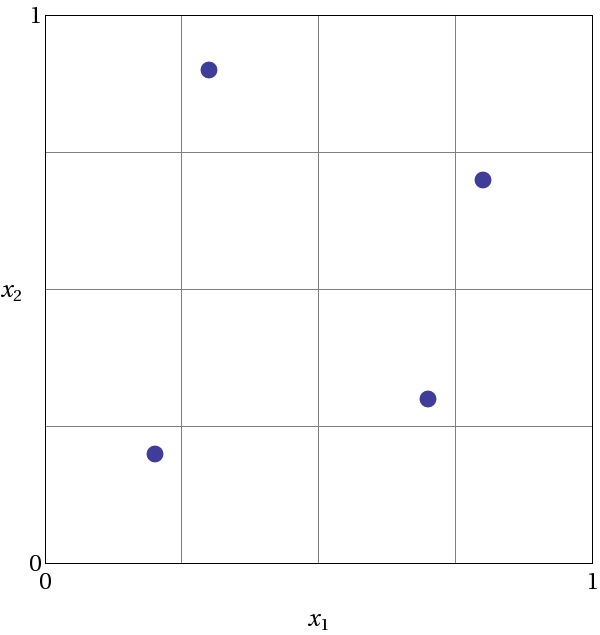
\includegraphics[scale=0.35]{images/lhs_graphic}
  \caption{An example of Latin hypercube sampling with four bins in
    design parameters $x_1$ and $x_2$. The dots
    are the sample sites.}
  \label{dace:figure01}
\end{figure}

The actual algorithm for generating Latin hypercube samples is more
complex than indicated by the description given above. For example,
the Latin hypercube sampling method implemented in the LHS
code~\cite{Swi04} takes into account a user-specified correlation
structure when selecting the sample sites. For more details on the
implementation of the LHS algorithm, see Reference~\cite{Swi04}.

In addition to Monte Carlo vs. LHS design choices, Dakota sampling
methods support options for incrementally-refined designs, generation
of approximately determinant-optimal (D-optimal) designs, and
selection of sample sizes to satisfy Wilks' criteria.

\subsection{Uncertainty Quantification Example using Sampling Methods}\label{uq:uncertainty1}

The input file in Figure~\ref{uq:figure01} 
demonstrates the use of Latin hypercube Monte Carlo sampling for
assessing probability of failure as measured by specified response
levels.  The two-variable Textbook example problem (see
Equation~\ref{additional:textbook_f}) will be used to demonstrate
the application of sampling methods for uncertainty quantification
where it is assumed that $x_1$ and $x_2$ are uniform uncertain
variables on the interval $[0,1]$. 

The number of samples to
perform is controlled with the \texttt{samples} specification, the
type of sampling algorithm to use is controlled with the
\texttt{sample\_type} specification, the levels used for computing
statistics on the response functions is specified with the
\texttt{response\_levels} input, and the \texttt{seed} specification
controls the sequence of the pseudo-random numbers generated by the
sampling algorithms. The input samples generated are shown in
Figure~\ref{uq:figure02} for the case where \texttt{samples} = 5 and
\texttt{samples} = 10 for both \texttt{random} ($\circ$) and 
\texttt{lhs} ($+$) sample types.

\begin{figure}[htbp!]
  \centering \begin{bigbox} \begin{small}
  \verbatimtabinput[8]{../../../test/examples-users/textbook_uq_sampling.in} \end{small} \end{bigbox}
\caption{Dakota input file for UQ example using LHS --
see \protect\path{dakota/share/dakota/examples/users/textbook_uq_sampling.in} }
\label{uq:figure01}
\end{figure}

\begin{figure}[htbp!]
  \centering
  \subfigure{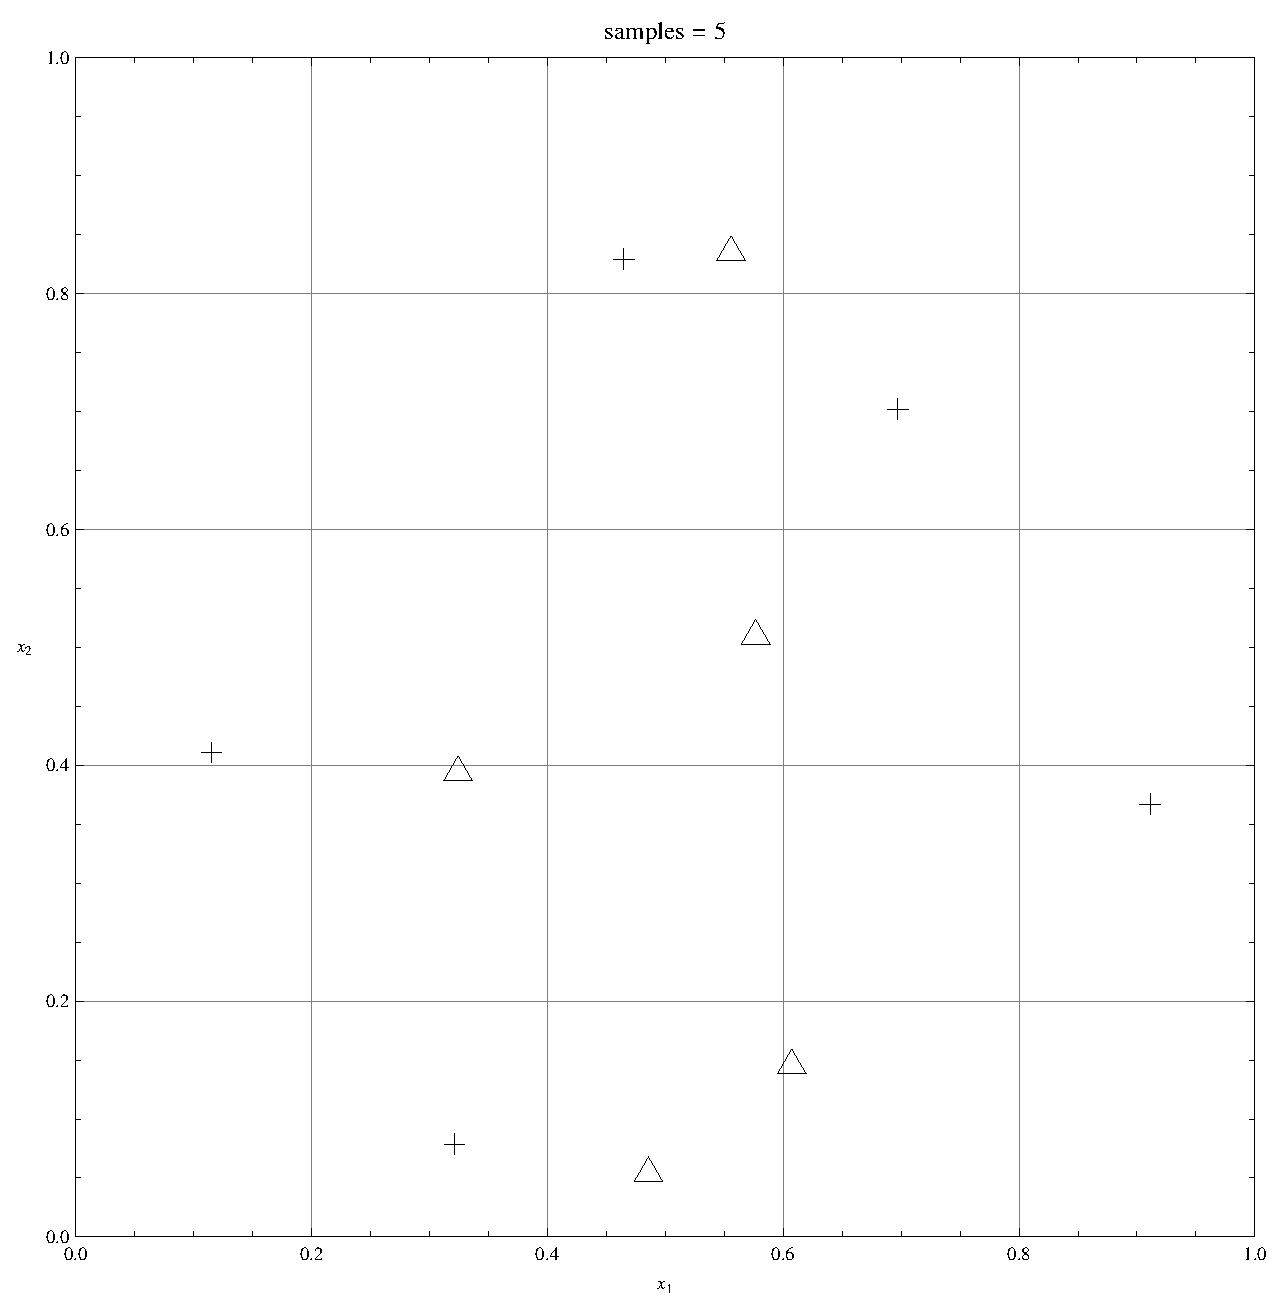
\includegraphics[scale=0.35]{images/input_samples5}}
  \subfigure{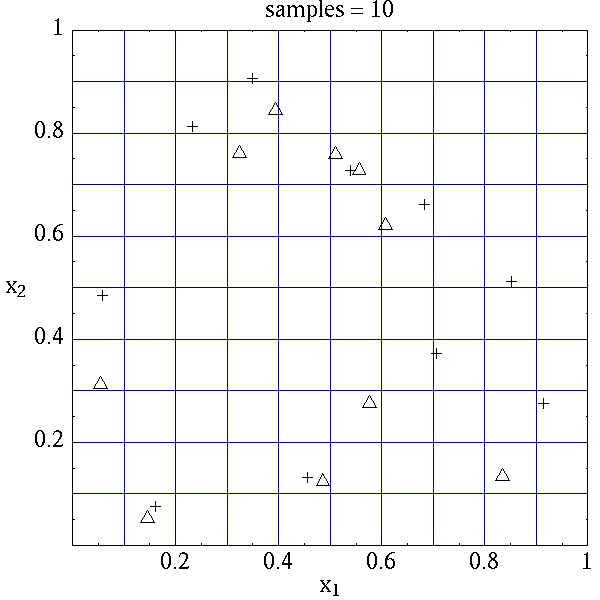
\includegraphics[scale=0.35]{images/input_samples10}}
  \caption{Distribution of input sample points for random ($\triangle$)
    and lhs ($+$) sampling for \texttt{samples=5} and \texttt{10}.}
  \label{uq:figure02}
\end{figure}

Latin hypercube sampling ensures full coverage of the range of the
input variables, which is often a problem with Monte Carlo sampling
when the number of samples is small. In the case of \texttt{samples =
5}, poor stratification is evident in $x_1$ as four out of the five
Monte Carlo samples are clustered in the range $0.35 < x_1 < 0.55$,
and the regions $x_1 < 0.3$ and $0.6 < x_1 < 0.9$ are completely
missed. For the case where \texttt{samples = 10}, some clustering in
the Monte Carlo samples is again evident with \texttt{4} samples in
the range $0.5 < x_1 < 0.55$. In both cases, the stratification with
LHS is superior. 

The response function statistics returned by Dakota
are shown in Figure~\ref{uq:figure03}. The first block of output
specifies the response sample means, sample standard deviations, and 
skewness and kurtosis.  The second block of output displays confidence 
intervals on the means and standard deviations of the responses.  
The third block defines Probability Density Function (PDF) histograms 
of the samples: the histogram bins are defined by the lower and upper 
values of the bin and the corresponding density for that bin.  
Note that these bin endpoints correspond to the \texttt{response\_levels} 
and/or \texttt{probability\_levels} defined by the user in the Dakota 
input file.  If there are just a few levels, these histograms may be coarse. 
Dakota does not do anything to optimize the bin size or spacing. 
Finally, the last section of the output defines the Cumulative Distribution 
Function (CDF) pairs.  In this case, 
\texttt{distribution cumulative} was specified for the response
functions, and Dakota presents the probability levels corresponding to the
specified response levels (\texttt{response\_levels}) that were set.
The
default \texttt{compute probabilities} was used. Alternatively,
Dakota could have provided CCDF pairings, reliability levels
corresponding to prescribed response levels, or response levels
corresponding to prescribed probability or reliability levels.

\begin{figure}[htbp!]
\centering
\begin{bigbox}
\begin{footnotesize}
\begin{verbatim}
Statistics based on 10 samples:

Sample moment statistics for each response function:
                            Mean           Std Dev          Skewness          Kurtosis
 response_fn_1  3.8383990322e-01  4.0281539886e-01  1.2404952971e+00  6.5529797327e-01
 response_fn_2  7.4798705803e-02  3.4686110941e-01  4.5716015887e-01 -5.8418924529e-01
 response_fn_3  7.0946176558e-02  3.4153246532e-01  5.2851897926e-01 -8.2527332042e-01

95% confidence intervals for each response function:
                    LowerCI_Mean      UpperCI_Mean    LowerCI_StdDev    UpperCI_StdDev
 response_fn_1  9.5683125821e-02  6.7199668063e-01  2.7707061315e-01  7.3538389383e-01
 response_fn_2 -1.7333078422e-01  3.2292819583e-01  2.3858328290e-01  6.3323317325e-01
 response_fn_3 -1.7337143113e-01  3.1526378424e-01  2.3491805390e-01  6.2350514636e-01

Probability Density Function (PDF) histograms for each response function:
PDF for response_fn_1:
          Bin Lower          Bin Upper      Density Value
          ---------          ---------      -------------
   2.3066424677e-02   1.0000000000e-01   3.8994678038e+00
   1.0000000000e-01   2.0000000000e-01   2.0000000000e+00
   2.0000000000e-01   6.0000000000e-01   5.0000000000e-01
   6.0000000000e-01   1.2250968624e+00   4.7992562123e-01
PDF for response_fn_2:
          Bin Lower          Bin Upper      Density Value
          ---------          ---------      -------------
  -3.5261164651e-01   1.0000000000e-01   1.1046998102e+00
   1.0000000000e-01   2.0000000000e-01   2.0000000000e+00
   2.0000000000e-01   6.0000000000e-01   5.0000000000e-01
   6.0000000000e-01   6.9844576220e-01   1.0157877573e+00
PDF for response_fn_3:
          Bin Lower          Bin Upper      Density Value
          ---------          ---------      -------------
  -3.8118095128e-01   1.0000000000e-01   1.2469321539e+00
   1.0000000000e-01   2.0000000000e-01   0.0000000000e+00
   2.0000000000e-01   6.0000000000e-01   7.5000000000e-01
   6.0000000000e-01   6.4526450977e-01   2.2092363423e+00

Level mappings for each response function:
Cumulative Distribution Function (CDF) for response_fn_1:
     Response Level  Probability Level  Reliability Index  General Rel Index
     --------------  -----------------  -----------------  -----------------
   1.0000000000e-01   3.0000000000e-01
   2.0000000000e-01   5.0000000000e-01
   6.0000000000e-01   7.0000000000e-01
Cumulative Distribution Function (CDF) for response_fn_2:
     Response Level  Probability Level  Reliability Index  General Rel Index
     --------------  -----------------  -----------------  -----------------
   1.0000000000e-01   5.0000000000e-01
   2.0000000000e-01   7.0000000000e-01
   6.0000000000e-01   9.0000000000e-01
Cumulative Distribution Function (CDF) for response_fn_3:
     Response Level  Probability Level  Reliability Index  General Rel Index
     --------------  -----------------  -----------------  -----------------
   1.0000000000e-01   6.0000000000e-01
   2.0000000000e-01   6.0000000000e-01
   6.0000000000e-01   9.0000000000e-01
\end{verbatim}
\end{footnotesize}
\end{bigbox}
\caption{Dakota response function statistics from UQ sampling example.}
\label{uq:figure03}
\end{figure}

In addition to obtaining statistical summary information of the type
shown in Figure~\ref{uq:figure03}, the results of LHS sampling also
include correlations. Four types of correlations are returned in the
output: simple and partial ``raw'' correlations, and simple and
partial ``rank'' correlations. The raw correlations refer to
correlations performed on the actual input and output data. Rank
correlations refer to correlations performed on the ranks of the data.
Ranks are obtained by replacing the actual data by the ranked values,
which are obtained by ordering the data in ascending order. For
example, the smallest value in a set of input samples would be given a
rank 1, the next smallest value a rank 2, etc. Rank correlations are
useful when some of the inputs and outputs differ greatly in
magnitude: then it is easier to compare if the smallest ranked input
sample is correlated with the smallest ranked output, for example.

Correlations are always calculated between two sets of sample data.
One can calculate correlation coefficients between two input
variables, between an input and an output variable (probably the most
useful), or between two output variables. The simple correlation
coefficients presented in the output tables are Pearson's correlation
coefficient, which is defined for two variables $x$ and $y$ as:
$\mathtt{Corr}(x,y) = \frac{\sum_{i}(x_{i}-\bar{x})(y_{i}-\bar{y})}
{\sqrt{\sum_{i}(x_{i}-\bar{x})^2\sum_{i}(y_{i}-\bar{y})^2}}$.
Partial correlation coefficients are similar to simple correlations,
but a partial correlation coefficient between two variables measures
their correlation while adjusting for the effects of the other
variables. For example, say one has a problem with two inputs and one
output; and the two inputs are highly correlated. Then the
correlation of the second input and the output may be very low after
accounting for the effect of the first input. The rank correlations
in Dakota are obtained using Spearman's rank correlation. Spearman's
rank is the same as the Pearson correlation coefficient except that it
is calculated on the rank data.

Figure~\ref{uq:figure04} shows an example of the correlation output
provided by Dakota for the input file in Figure~\ref{uq:figure01}.
Note that these correlations are presently only available when one
specifies \texttt{lhs} as the sampling method under \texttt{sampling}.
Also note that the simple and partial correlations should be similar in most
cases (in terms of values of correlation coefficients). This is
because we use a default ``restricted pairing'' method in the LHS
routine which forces near-zero correlation amongst uncorrelated
inputs.

\begin{figure}[htbp!]
\centering
\begin{bigbox}
\begin{small}
\begin{verbatim}
Simple Correlation Matrix between input and output:
                       x1           x2 response_fn_1 response_fn_2 response_fn_3
          x1  1.00000e+00
          x2 -7.22482e-02  1.00000e+00
response_fn_1 -7.04965e-01 -6.27351e-01  1.00000e+00
response_fn_2  8.61628e-01 -5.31298e-01 -2.60486e-01  1.00000e+00
response_fn_3 -5.83075e-01  8.33989e-01 -1.23374e-01 -8.92771e-01  1.00000e+00

Partial Correlation Matrix between input and output:
             response_fn_1 response_fn_2 response_fn_3
          x1 -9.65994e-01  9.74285e-01 -9.49997e-01
          x2 -9.58854e-01 -9.26578e-01  9.77252e-01

Simple Rank Correlation Matrix between input and output:
                       x1           x2 response_fn_1 response_fn_2 response_fn_3
          x1  1.00000e+00
          x2 -6.66667e-02  1.00000e+00
response_fn_1 -6.60606e-01 -5.27273e-01  1.00000e+00
response_fn_2  8.18182e-01 -6.00000e-01 -2.36364e-01  1.00000e+00
response_fn_3 -6.24242e-01  7.93939e-01 -5.45455e-02 -9.27273e-01  1.00000e+00

Partial Rank Correlation Matrix between input and output:
             response_fn_1 response_fn_2 response_fn_3
          x1 -8.20657e-01  9.74896e-01 -9.41760e-01
          x2 -7.62704e-01 -9.50799e-01  9.65145e-01
\end{verbatim}
\end{small}
\end{bigbox}
\caption{Correlation results using LHS Sampling.}
\label{uq:figure04}
\end{figure}

Finally, note that the LHS package can be used for design of
experiments over design and state variables by including an active
view override in the variables specification section of the Dakota
input file (see Section~\ref{variables:mixedview}). Then, instead of
iterating on only the uncertain variables, the LHS package will sample
over all of the active variables. In the \texttt{active all} view,
continuous design and continuous state variables are treated as having
uniform probability distributions within their upper and lower bounds,
discrete design and state variables are sampled uniformly from within
their sets or ranges, and any uncertain variables are sampled within
their specified probability distributions.

\subsection{Incremental Sampling}\label{uq:incremental}

In many situations, one may run an initial sample set and then need to
perform further sampling to get better estimates of the mean,
variance, and percentiles, and to obtain more comprehensive sample
coverage. We call this capability incremental sampling.  Typically, a
Dakota restart file (\path{dakota.rst}) would be available from the
original sample, so only the newly generated samples would need to be
evaluated.  Incremental sampling supports continuous uncertain
variables and discrete uncertain variables such as discrete
distributions (e.g.  binomial, Poisson, etc.) as well as histogram
variables and uncertain set types.

There are two cases, incremental random and incremental Latin
hypercube sampling, with incremental LHS being the most common.  One
major advantage of LHS incremental sampling is that it maintains the
stratification and correlation structure of the original LHS sample.
That is, if one generated two independent LHS samples and simply
merged them, the calculation of the accuracy of statistical measures
such as the mean and the variance would be slightly
incorrect. However, in the incremental case, the full sample (double
the original size) is a Latin Hypercube sample itself and statistical
measures and their accuracy can be properly calculated. The
incremental sampling capability is most useful when one is starting
off with very small samples. Once the sample size is more than a few
hundred, the benefit of incremental sampling diminishes.

\begin{enumerate}

\item Incremental random sampling: With incremental random sampling,
  the original sample set with $N1$ samples must be generated using
  \texttt{sample\_type = random} and \texttt{samples = N1}.  Then, the
  user can duplicate the Dakota input file and add
  \texttt{refinement\_samples = N2} with the number of new samples
  $N2$ to be added.  Random incremental sampling does not require a
  doubling of samples each time. Thus, the user can specify any number
  of \texttt{refinement\_samples} (from an additional one sample to a
  large integer).

  For example, if the first sample has 50 samples, and 10 more samples
  are desired, the second Dakota run should specify \texttt{samples =
    50}, \texttt{refinement\_samples = 10}.  In this situation, only
  10 new samples will be generated, and the final statistics will be
  reported at the end of the study both for the initial 50 samples and
  for the full sample of 60. The command line syntax for
  running the second sample is \texttt{dakota -i input60.in -r
    dakota.50.rst} where \texttt{input60.in} is the input file with
  the refinement samples specification and \path{dakota.50.rst} is
  the restart file containing the initial 50 samples.  Note that if
  the restart file has a different name, that is fine; the correct
  restart file name should be used.

  This process can be repeated if desired,arbitrarily extending the
  total sample size each time, e.g, \texttt{samples = 50},
  \texttt{refinement\_samples = 10  3  73  102}.

\item Incremental Latin hypercube sampling: With incremental LHS
  sampling, the original sample set with $N1$ samples must be
  generated using \texttt{sample\_type = lhs} and \texttt{samples =
    N1}.  Then, the user can duplicate the Dakota input file and add
  \texttt{refinement\_samples = N1}.  The sample size must double each
  time, so the first set of refinement samples must be the same size
  as the initial set.  That is, if one starts with a very small sample
  size of 10, then one can use the incremental sampling capability to
  generate sample sizes of 20, 40, 80, etc.

  For example, if the first sample has 50 samples, in the second
  Dakota run, the number of refinement samples should be set to 50 for
  a total of 100. In this situation, only 50 new samples will be
  generated, and at the end of the study final statistics will be reported 
  both for the initial 50 samples and for the full sample of 100. The command 
  line syntax for running the second sample
  is \texttt{dakota -i input100.in -r dakota.50.rst}, where
  \path{input100.in} is the input file with the incremental sampling
  specification and \path{dakota.50.rst} is the restart file
  containing the initial 50 samples.  Note that if the restart file
  has a different name, that is fine; the correct restart file name
  should be used.

  This process can be repeated if desired, doubling the total sample
  size each time, e.g, \texttt{samples = 50},
  \texttt{refinement\_samples = 50  100  200  400}.

\end{enumerate}

\subsection{Principal Component Analysis} 
As of Dakota 6.3, we added a capability to perform 
Principal Component Analysis on field response data when 
using LHS sampling.  Principal components analysis (PCA) 
is a data reduction method and allows one to express an 
ensemble of field data with a set of principal components 
responsible for the spread of that data.

Dakota can calculate the principal components of the response matrix of
N samples * L responses (the field response of length L) 
using the keyword \texttt{principal\_components}.
The Dakota implementation is under active development:  the PCA capability
may ultimately be specified elsewhere or used in different ways.
For now, it is performed as a post-processing analysis based on a set of 
Latin Hypercube samples.
 
If the user specifies LHS sampling with field data responses and also 
specifies \texttt{principal\_components}, Dakota will calculate the principal
components by calculating the eigenvalues and eigenvectors of a centered 
data matrix.   
Further, if the user specifies \texttt{percent\_variance\_explained} = 0.99, 
the number of components that accounts for at least 99 percent of the variance 
in the responses will be retained.  The default for this percentage is 0.95.  
In many applications, only a few principal components explain the majority 
of the variance, resulting in significant data reduction.
The principal components are written to a file, \path{princ_comp.txt}.
Dakota also uses the principal components to create a surrogate model by 
representing the overall response as weighted sum of M principal components, 
where the weights will be determined by Gaussian processes which are a function 
of the input uncertain variables.  This reduced form then can be used for 
sensitivity analysis, calibration, etc.  

\subsection{Wilks-based Sample Sizes}\label{uq:wilks}

Most of the sampling methods require the user to specify the number of
samples in advance.  However, if one specifies \texttt{random} sampling,
one can use an approach developed by Wilks\cite{Wilks} to determine
the number of samples that ensures a particular confidence level in
a percentile of interest.  The Wilks method of computing the number
of samples to execute for a random sampling study is based on order
statistics, eg considering the outputs ordered from smallest to largest
\cite{Wilks,Nutt04}.  Given a \texttt{probability\_level}, $\alpha$,
and \texttt{confidence\_level}, $\beta$, the Wilks calculation determines
the minimum number of samples required such that there is $(\beta*100)$\%
confidence that the $(\alpha*100)$\%-ile of the uncertain distribution
on model output will fall below the actual $(\alpha*100)$\%-ile given
by the sample.  To be more specific, if we wish to calculate the $95\%$
confidence limit on the $95^{th}$ percentile, Wilks indicates that 59
samples are needed.  If we order the responses and take the largest one,
that value defines a tolerance limit on the 95th percentile:  we have a
situation where $95\%$ of the time, the $95^{th}$ percentile will fall at
or below that sampled value.  This represents a \texttt{one\_sided\_upper}
treatment applicable to the largest output value.  This treatment
can be reversed to apply to the lowest output value by using the
\texttt{one\_sided\_lower} option, and further expansion to include an
interval containing both the smallest and the largest output values in
the statistical statement can be specified via the \texttt{two\_sided}
option.  Additional generalization to higher order statistics, eg a
statement applied to the N largest outputs (\texttt{one\_sided\_upper}) or the
N smallest and N largest outputs (\texttt{two\_sided}), can be specified
using the \texttt{order} option along with value N.

\section{Reliability Methods}\label{uq:reliability}

Reliability methods provide an alternative approach to uncertainty
quantification which can be less computationally demanding than
sampling techniques. Reliability methods for uncertainty
quantification are based on probabilistic approaches that compute
approximate response function distribution statistics based on
specified uncertain variable distributions. These response statistics
include response mean, response standard deviation, and cumulative or
complementary cumulative distribution functions (CDF/CCDF). These
methods are often more efficient at computing statistics in the tails
of the response distributions (events with low probability) than
sampling based approaches since the number of samples required to
resolve a low probability can be prohibitive.

The methods all answer the fundamental question: ``Given a set of
uncertain input variables, $\mathbf{X}$, and a scalar response
function, $g$, what is the probability that the response function is
below or above a certain level, $\bar{z}$?'' The former can be written
as $P[g(\mathbf{X}) \le \bar{z}] = \mathit{F}_{g}(\bar{z})$ where
$\mathit{F}_{g}(\bar{z})$ is the cumulative distribution function
(CDF) of the uncertain response $g(\mathbf{X})$ over a set of response
levels. The latter can be written as $P[g(\mathbf{X}) > \bar{z}]$ and
defines the complementary cumulative distribution function (CCDF).

This probability calculation involves a multi-dimensional integral
over an irregularly shaped domain of interest, $\mathbf{D}$, where
$g(\mathbf{X}) < z$ as displayed in Figure~\ref{uq:figure05} for the
case of two variables. The reliability methods all involve the
transformation of the user-specified uncertain variables,
$\mathbf{X}$, with probability density function, $p(x_1,x_2)$, which
can be non-normal and correlated, to a space of independent Gaussian
random variables, $\mathbf{u}$, possessing a mean value of zero and
unit variance (i.e., standard normal variables). The region of
interest, $\mathbf{D}$, is also mapped to the transformed space to
yield, $\mathbf{D_{u}}$ , where $g(\mathbf{U}) < z$ as shown in
Figure~\ref{uq:figure06}. The Nataf transformation~\cite{Der86},
which is identical to the Rosenblatt transformation~\cite{Ros52} in
the case of independent random variables, is used in Dakota to
accomplish this mapping. This transformation is performed to make the
probability calculation more tractable. In the transformed space,
probability contours are circular in nature as shown in
Figure~\ref{uq:figure06} unlike in the original uncertain variable
space, Figure~\ref{uq:figure05}. Also, the multi-dimensional integrals
can be approximated by simple functions of a single parameter,
$\beta$, called the reliability index. $\beta$ is the minimum
Euclidean distance from the origin in the transformed space to the
response surface. This point is also known as the most probable point
(MPP) of failure. Note, however, the methodology is equally applicable
for generic functions, not simply those corresponding to failure
criteria; this nomenclature is due to the origin of these methods
within the disciplines of structural safety and reliability.
Note that there are local and global reliability methods. The majority 
of the methods available are local, meaning that a local optimization 
formulation is used to locate one MPP. In contrast, global methods
can find multiple MPPs if they exist.
\begin{figure}[htbp!]
  \centering
  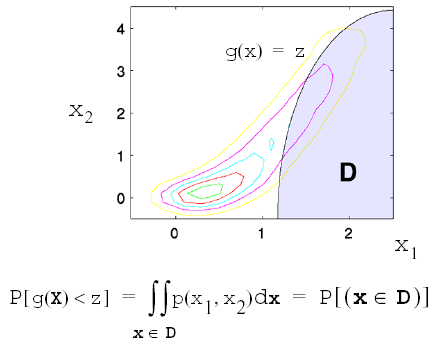
\includegraphics[scale=0.75]{images/cdf_orig_graphic}
  \caption{Graphical depiction of calculation of cumulative
    distribution function in the original uncertain variable space.}
  \label{uq:figure05}
\end{figure}

\begin{figure}[htbp!]
  \centering
  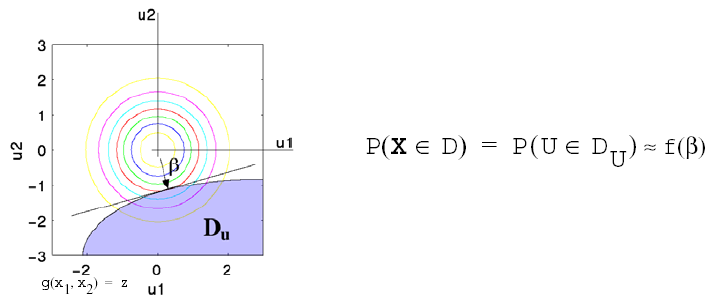
\includegraphics[scale=0.75]{images/cdf_tran_graphic}
  \caption{Graphical depiction of integration for the calculation of
    cumulative distribution function in the transformed uncertain
    variable space.}
  \label{uq:figure06}
\end{figure}

\subsection{Local Reliability Methods}\label{uq:reliability:local}

The Dakota Theory Manual~\cite{TheoMan} provides the algorithmic
details for the local reliability methods, including the Mean Value
method and the family of most probable point (MPP) search methods.


\subsubsection{Method mapping} \label{uq:reliability:local:map}

Given settings for limit state approximation, approximation order,
integration approach, and other details presented to this point, it is
evident that the number of algorithmic combinations is high.
Table~\ref{tab:rel_meth_map} provides a succinct mapping for some of
these combinations to common method names from the reliability
literature, where blue indicates the most well-known combinations and
gray indicates other supported combinations.
\begin{table}
\centering
\caption{Mapping from Dakota options to standard reliability methods.}
\label{tab:rel_meth_map}
\begin{tabular}{|c|c|c|}
\hline
& \multicolumn{2}{c|}{Order of approximation and integration} \\ \cline{2-3}
MPP search      & First order & Second order                        \\ \hline
none            & \cellcolor{blue}\textcolor{white}{MVFOSM}
                & \cellcolor[gray]{0.5}\textcolor{black}{MVSOSM}   \\ \hline
x\_taylor\_mean & \cellcolor{blue}\textcolor{white}{AMV}
                & \cellcolor[gray]{0.5}\textcolor{black}{AMV$^2$}  \\ \hline
u\_taylor\_mean & \cellcolor[gray]{0.5}\textcolor{black}{u-space AMV}
                & \cellcolor[gray]{0.5}\textcolor{black}{u-space AMV$^2$} \\
\hline
x\_taylor\_mpp  & \cellcolor{blue}\textcolor{white}{AMV+}
                & \cellcolor[gray]{0.5}\textcolor{black}{AMV$^2$+} \\ \hline
u\_taylor\_mpp  & \cellcolor[gray]{0.5}\textcolor{black}{u-space AMV+}
                & \cellcolor[gray]{0.5}\textcolor{black}{u-space AMV$^2$+} \\
\hline
x\_two\_point   & \cellcolor{blue}\textcolor{white}{TANA}
                & \cellcolor[gray]{0.5}                             \\ \hline
u\_two\_point   & \cellcolor[gray]{0.5}\textcolor{black}{u-space TANA}
                & \cellcolor[gray]{0.5}                             \\ \hline
no\_approx      & \cellcolor{blue}\textcolor{white}{FORM}
                & \cellcolor{blue}\textcolor{white}{SORM}           \\ \hline
\end{tabular}
\end{table}

Within the Dakota specification (refer to \texttt{local\_reliability}
in the keywords section of the Reference Manual~\cite{RefMan})
within the Reference Manual), the MPP search and integration order
selections are explicit in the method specification, but the order of
the approximation is inferred from the associated response
specification (as is done with local taylor series approximations
described in Section~\ref{models:surf:taylor}). Thus, reliability
methods do not have to be synchronized in approximation and
integration order as shown in the table; however, it is often
desirable to do so.


\subsection{Global Reliability Methods}\label{uq:reliability:global}

Global reliability methods are designed to handle nonsmooth and
multimodal failure surfaces, by creating global approximations based
on Gaussian process models. They accurately resolve a particular
contour of a response function and then estimate probabilities using
multimodal adaptive importance sampling.

The global reliability method in Dakota is called 
Efficient Global Reliability Analysis (EGRA) ~\cite{Bichon2008}. 
The name is due to its 
roots in efficient global optimization (EGO) ~\cite{Jon98,Hua06}.
The main idea in EGO-type optimization methods is that a global 
approximation is made of the underlying function. This approximation, 
which is a Gaussian process model, is used to guide the search by finding 
points which maximize the expected improvement function (EIF). 
The EIF is used to select the location at which a new training point should be
added to the Gaussian process model by maximizing the amount of improvement 
in the objective function that can be expected by adding that point.
A point could be expected to produce an improvement in the objective function 
if its predicted value is better than the current best solution, or if the 
uncertainty in its prediction is such that the probability of it producing
a better solution is high.
Because the uncertainty is higher in regions of the design space with fewer
observations, this provides a balance between exploiting areas of the
design space that predict good solutions, and exploring areas where more
information is needed.

The general procedure of these EGO-type methods is:
\begin{enumerate}
\item Build an initial Gaussian process model of the objective function.
%\item Use cross validation to ensure that the GP model is satisfactory.
\item Find the point that maximizes the EIF.
      If the EIF value at this point is sufficiently small, stop.
\item Evaluate the objective function at the point where the EIF is maximized.
      Update the Gaussian process model using this new point.
      Go to Step 2.
\end{enumerate}

Gaussian process (GP) models are used because
they provide not just a predicted value at an unsampled point, but also an
estimate of the prediction variance.
This variance gives an indication of the uncertainty in the GP model, which
results from the construction of the covariance function.
This function is based on the idea that when input points are near one another,
the correlation between their corresponding outputs will be high.
As a result, the uncertainty associated with the model's predictions will be
small for input points which are near the points used to train the model,
and will increase as one moves further from the training points.

The expected improvement function is used in EGO algorithms 
to select the location at which a new training point should be added.
The EIF is defined as the expectation that any point in the search
space will provide a better solution than the current best solution
based on the expected values and variances predicted by the GP model.
It is important to understand how the use of this EIF leads to optimal
solutions. The EIF indicates how much the objective function value at 
a new potential location 
is expected to be less than the predicted value at the current best solution.
Because the GP model provides a Gaussian distribution at each predicted
point, expectations can be calculated.
Points with good expected values and even a small variance will
have a significant expectation of producing a better solution (exploitation),
but so will points that have relatively poor expected values and greater
variance (exploration).
 
The application of EGO to reliability analysis, however, is made more
complicated due to the inclusion of equality constraints.
In forward reliability analysis, the response function appears as a 
constraint rather than the objective. That is, we want to satisfy 
the constraint that the response equals a threshold value 
and is on the limit state:  $G({\bf u})\!=\!\bar{z}$.
Therefore, the EIF function was modified to focus on feasibility, 
and instead of using an expected improvement function, we use an 
expected feasibility function (EFF) ~\cite{Bichon2008}. 
The EFF provides an indication of how well the response is expected 
to satisfy the equality constraint. 
Points where the expected value is close to the threshold
($\mu_G\!\approx\!\bar{z}$) and points with a large uncertainty in the
prediction will have large expected feasibility values.

The general outline of the EGRA algorithm is as follows:  LHS sampling 
is used to generate a small number of samples from the true response 
function. Then, an initial Gaussian process model is constructed. 
Based on the EFF, the point with maximum EFF is found using 
the global optimizer DIRECT. The true response function is then 
evaluated at this new point, and this point is added to the sample set 
and the process of building a new GP model and maximizing the EFF is 
repeated until the maximum EFF is small. At this stage, the GP model 
is accurate in the vicinity of the limit state. The GP model 
is then used to calculate the probability of failure 
using multimodal importance sampling, which is explained below. 

One method to calculate the probability of failure is 
to directly perform the probability 
integration numerically by sampling the response function.
Sampling methods can be 
prohibitively expensive because they generally require a large 
number of response function evaluations.
Importance sampling methods reduce this expense by focusing the samples in 
the important regions of the uncertain space.
They do this by centering the sampling density function at the MPP rather
than at the mean.
This ensures the samples will lie the region of interest, 
thus increasing the efficiency of the sampling method.
Adaptive importance sampling (AIS) further improves the efficiency by 
adaptively updating the sampling density function.
Multimodal adaptive importance sampling~\cite{Dey98} is a 
variation of AIS that allows for the use of multiple sampling densities 
making it better suited for cases where multiple sections of the limit state 
are highly probable.

Note that importance sampling methods require that the location of at least 
one MPP be known because it is used to center the initial sampling density.
However, current gradient-based, local search methods used in MPP search may 
fail to converge or may converge to poor solutions for 
highly nonlinear problems, possibly making these methods inapplicable.
The EGRA algorithm described above does 
not depend on the availability of accurate gradient information, making
convergence more reliable for nonsmooth response functions.
Moreover, EGRA has the ability to locate multiple failure points, which 
can provide multiple starting points and thus a good multimodal sampling density for the initial steps of multimodal AIS. The probability assessment 
using multimodal AIS thus incorporates probability of failure at 
multiple points.

\subsection{Uncertainty Quantification Examples using Reliability Analysis} \label{uq:reliability:ex}

%Reliability methods provide an alternative approach to uncertainty
%quantification which can be less computationally demanding than
%sampling techniques. 

In summary, the user can choose to perform either forward (RIA) or
inverse (PMA) mappings when performing a reliability analysis. With
either approach, there are a variety of methods from which to choose
in terms of limit state approximations (MVFOSM, MVSOSM, x-/u-space
AMV, x-/u-space AMV$^2$, x-/u-space AMV+, x-/u-space AMV$^2$+,
x-/u-space TANA, and FORM/SORM), probability integrations
(first-order or second-order), limit state Hessian selection
(analytic, finite difference, BFGS, or SR1), and MPP optimization
algorithm (SQP or NIP) selections.

All reliability methods output approximate values of the CDF/CCDF
response-probability-reliability levels for prescribed response levels
(RIA) or prescribed probability or reliability levels (PMA). In
addition, mean value methods output estimates of the response means
and standard deviations as well as importance factors that attribute
variance among the set of uncertain variables (provided a nonzero
response variance estimate).

\subsubsection{Mean-value Reliability with Textbook}
\label{uq:examples:mv}

Figure~\ref{uq:examples:mv_input} shows the Dakota input file for an
example problem that demonstrates the simplest reliability method,
called the mean value method (also referred to as the Mean Value First
Order Second Moment method). It is specified with method keyword
\texttt{local\_reliability}. This method calculates the mean and
variance of the response function based on information about the mean
and variance of the inputs and gradient information at the mean of the
inputs. The mean value method is extremely cheap computationally (only
five runs were required for the textbook function), but can be quite
inaccurate, especially for nonlinear problems and/or problems with
uncertain inputs that are significantly non-normal. More detail on the
mean value method can be found in the Local Reliability Methods
section of the Dakota Theory Manual~\cite{TheoMan}, and more detail on
reliability methods in general (including the more advanced methods)
is found in Section~\ref{uq:reliability}.

Example output from the mean value method is displayed in
Figure~\ref{uq:examples:mv_results}. Note that since the mean of both
inputs is 1, the mean value of the output for response 1 is zero.
However, the mean values of the constraints are both 0.5.  The mean
value results indicate that variable x1 is more important in
constraint 1 while x2 is more important in constraint 2, which is the
case based on Equation~\ref{additional:textbook_f}.  The importance
factors are not available for the first response as the standard
deviation is zero.

\begin{figure}[htbp!]
  \centering
  \begin{bigbox}
    \begin{small}
      \verbatimtabinput[8]{../../../test/examples-users/textbook_uq_meanvalue.in}
    \end{small}
  \end{bigbox}
  \caption{Mean Value Reliability Method: the Dakota input file -- see
    \protect\path{dakota/share/dakota/examples/users/textbook_uq_meanvalue.in}
  }
  \label{uq:examples:mv_input}
\end{figure}

\begin{figure}[htbp!]
\centering
\begin{bigbox}
\begin{small}
\begin{verbatim}
MV Statistics for response_fn_1:
  Approximate Mean Response                  =  0.0000000000e+00
  Approximate Standard Deviation of Response =  0.0000000000e+00
  Importance Factors not available.
MV Statistics for response_fn_2:
  Approximate Mean Response                  =  5.0000000000e-01
  Approximate Standard Deviation of Response =  1.0307764064e+00
  Importance Factor for TF1ln                =  9.4117647059e-01
  Importance Factor for TF2ln                =  5.8823529412e-02
MV Statistics for response_fn_3:
  Approximate Mean Response                  =  5.0000000000e-01
  Approximate Standard Deviation of Response =  1.0307764064e+00
  Importance Factor for TF1ln                =  5.8823529412e-02
  Importance Factor for TF2ln                =  9.4117647059e-01
\end{verbatim}
\end{small}
\end{bigbox}
\caption{Results of the Mean Value Method on the Textbook Function}
\label{uq:examples:mv_results}
\end{figure}

\subsubsection{FORM Reliability with Lognormal Ratio}

This example quantifies the uncertainty in the ``log ratio'' response
function:
\begin{equation}
g(x_1,x_2) = \frac{x_1}{x_2}
\end{equation}
by computing approximate response statistics using reliability
analysis to determine the response cumulative distribution function:
\begin{equation}
P[g(x_1,x_2) < \bar{z}]
\end{equation}
where $X_1$ and $X_2$ are identically distributed lognormal random
variables with means of \texttt{1}, standard deviations of
\texttt{0.5}, and correlation coefficient of \texttt{0.3}.

A Dakota input file showing RIA using FORM (option 7 in limit state
approximations combined with first-order integration) is listed in
Figure~\ref{uq:rel_input_form}.
The user first specifies the \texttt{local\_reliability}
method, followed by the MPP search approach and integration order. In
this example, we specify \texttt{mpp\_search no\_approx} and utilize
the default first-order integration to select FORM. Finally, the user
specifies response levels or probability/reliability levels to
determine if the problem will be solved using an RIA approach or a PMA
approach. In the example figure of~\ref{uq:rel_input_form}, we use
RIA by specifying a range of \texttt{response\_levels} for the
problem. The resulting output for this input is shown in
Figure~\ref{uq:rel_output_form}, with probability and reliability
levels listed for each response level. Figure~\ref{uq:rel_form_compare} 
shows that FORM compares favorably to an exact analytic solution for
this problem. Also note that FORM does have some error in the
calculation of CDF values for this problem, but it is a very small
error (on the order of e-11), much smaller than the error obtained
when using a Mean Value method, which will be discussed next.
\begin{figure}[htbp!]
  \centering
  \begin{bigbox}
    \begin{small}
      \verbatimtabinput[8]{../../../test/examples-users/logratio_uq_reliability.in}
    \end{small}
  \end{bigbox}
\caption{Dakota input file for Reliability UQ example using FORM --
see \protect\path{dakota/share/dakota/examples/users/logratio_uq_reliability.in} }
\label{uq:rel_input_form}
\end{figure}

\begin{figure}[htbp!]
\centering
\begin{bigbox}
\begin{small}
\begin{verbatim}
Cumulative Distribution Function (CDF) for response_fn_1:
     Response Level  Probability Level  Reliability Index
     --------------  -----------------  -----------------
   4.0000000000e-01   4.7624085962e-02   1.6683404020e+00
   5.0000000000e-01   1.0346525475e-01   1.2620507942e+00
   5.5000000000e-01   1.3818404972e-01   1.0885143628e+00
   6.0000000000e-01   1.7616275822e-01   9.3008801339e-01
   6.5000000000e-01   2.1641741368e-01   7.8434989943e-01
   7.0000000000e-01   2.5803428381e-01   6.4941748143e-01
   7.5000000000e-01   3.0020938124e-01   5.2379840558e-01
   8.0000000000e-01   3.4226491013e-01   4.0628960782e-01
   8.5000000000e-01   3.8365052982e-01   2.9590705956e-01
   9.0000000000e-01   4.2393548232e-01   1.9183562480e-01
   1.0000000000e+00   5.0000000000e-01   6.8682233460e-12
   1.0500000000e+00   5.3539344228e-01  -8.8834907167e-02
   1.1500000000e+00   6.0043460094e-01  -2.5447217462e-01
   1.2000000000e+00   6.3004131827e-01  -3.3196278078e-01
   1.2500000000e+00   6.5773508987e-01  -4.0628960782e-01
   1.3000000000e+00   6.8356844630e-01  -4.7770089473e-01
   1.3500000000e+00   7.0761025532e-01  -5.4641676380e-01
   1.4000000000e+00   7.2994058691e-01  -6.1263331274e-01
   1.5000000000e+00   7.6981945355e-01  -7.3825238860e-01
   1.5500000000e+00   7.8755158269e-01  -7.9795460350e-01
   1.6000000000e+00   8.0393505584e-01  -8.5576118635e-01
   1.6500000000e+00   8.1906005158e-01  -9.1178881995e-01
   1.7000000000e+00   8.3301386860e-01  -9.6614373461e-01
   1.7500000000e+00   8.4588021938e-01  -1.0189229206e+00
\end{verbatim}
\end{small}
\end{bigbox}
\caption{Output from Reliability UQ example using FORM.}
\label{uq:rel_output_form}
\end{figure}

\begin{figure}[htbp!]
  \centering
  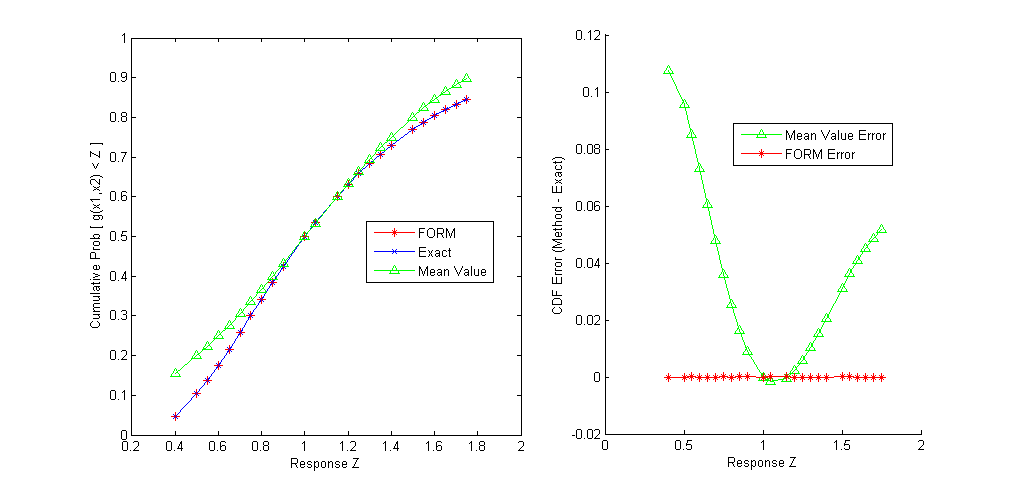
\includegraphics[scale=0.5]{images/cdf_form}
\caption{Comparison of the cumulative distribution function (CDF) computed by
FORM, the Mean Value method, and the exact CDF for $g(x_1,x_2)=\frac{x_1}{x_2}$}
\label{uq:rel_form_compare}
\end{figure}

If the user specifies \texttt{local\_reliability} as a method with no
additional specification on how to do the MPP search (for example, by
commenting out {\tt mpp\_search no\_approx} in
Figure~\ref{uq:rel_input_form}), then no MPP search is done: the Mean
Value method is used. The mean value results are shown in
Figure~\ref{uq:rel_output_mv} and consist of approximate mean and
standard deviation of the response, the importance factors for each
uncertain variable, and approximate probability/reliability levels for
the prescribed response levels that have been inferred from the
approximate mean and standard deviation (see Mean Value section in
Reliability Methods Chapter of Dakota Theory
Manual~\cite{TheoMan}). It is evident that the statistics are
considerably different from the fully converged FORM results; however,
these rough approximations are also much less expensive to
calculate. The importance factors are a measure of the sensitivity of
the response function(s) to the uncertain input variables. A
comparison of the mean value results with the FORM results is shown in
Figure~\ref{uq:rel_form_compare}. The mean value results are not
accurate near the tail values of the CDF, and can differ from the
exact solution by as much as 0.11 in CDF estimates. A comprehensive
comparison of various reliability methods applied to the logratio
problem is provided in ~\cite{Eld06a}.

\begin{figure}[htbp!]
\begin{bigbox}
\begin{small}
\begin{verbatim}
MV Statistics for response_fn_1:
  Approximate Mean Response                  =  1.0000000000e+00
  Approximate Standard Deviation of Response =  5.9160798127e-01
  Importance Factor for TF1ln                =  7.1428570714e-01
  Importance Factor for TF2ln                =  7.1428572143e-01
  Importance Factor for TF1ln     TF2ln      = -4.2857142857e-01
Cumulative Distribution Function (CDF) for response_fn_1:
     Response Level  Probability Level  Reliability Index  General Rel Index
     --------------  -----------------  -----------------  -----------------
   4.0000000000e-01   1.5524721837e-01   1.0141851006e+00   1.0141851006e+00
   5.0000000000e-01   1.9901236093e-01   8.4515425050e-01   8.4515425050e-01
   5.5000000000e-01   2.2343641149e-01   7.6063882545e-01   7.6063882545e-01
   6.0000000000e-01   2.4948115037e-01   6.7612340040e-01   6.7612340040e-01
   6.5000000000e-01   2.7705656603e-01   5.9160797535e-01   5.9160797535e-01
   7.0000000000e-01   3.0604494093e-01   5.0709255030e-01   5.0709255030e-01
   7.5000000000e-01   3.3630190949e-01   4.2257712525e-01   4.2257712525e-01
   8.0000000000e-01   3.6765834596e-01   3.3806170020e-01   3.3806170020e-01
   8.5000000000e-01   3.9992305332e-01   2.5354627515e-01   2.5354627515e-01
   9.0000000000e-01   4.3288618783e-01   1.6903085010e-01   1.6903085010e-01
   1.0000000000e+00   5.0000000000e-01   0.0000000000e+00   0.0000000000e+00
   1.0500000000e+00   5.3367668035e-01  -8.4515425050e-02  -8.4515425050e-02
   1.1500000000e+00   6.0007694668e-01  -2.5354627515e-01  -2.5354627515e-01
   1.2000000000e+00   6.3234165404e-01  -3.3806170020e-01  -3.3806170020e-01
   1.2500000000e+00   6.6369809051e-01  -4.2257712525e-01  -4.2257712525e-01
   1.3000000000e+00   6.9395505907e-01  -5.0709255030e-01  -5.0709255030e-01
   1.3500000000e+00   7.2294343397e-01  -5.9160797535e-01  -5.9160797535e-01
   1.4000000000e+00   7.5051884963e-01  -6.7612340040e-01  -6.7612340040e-01
   1.5000000000e+00   8.0098763907e-01  -8.4515425050e-01  -8.4515425050e-01
   1.5500000000e+00   8.2372893005e-01  -9.2966967555e-01  -9.2966967555e-01
   1.6000000000e+00   8.4475278163e-01  -1.0141851006e+00  -1.0141851006e+00
   1.6500000000e+00   8.6405064339e-01  -1.0987005257e+00  -1.0987005257e+00
   1.7000000000e+00   8.8163821351e-01  -1.1832159507e+00  -1.1832159507e+00
   1.7500000000e+00   8.9755305196e-01  -1.2677313758e+00  -1.2677313758e+00
\end{verbatim}
\end{small}
\end{bigbox}
\caption{Output from Reliability UQ example using mean value.}
\label{uq:rel_output_mv}
\end{figure}

Additional reliability analysis and design results are provided in 
Sections~\ref{additional:logratio}-\ref{additional:steel_column}.


\section{Stochastic Expansion Methods}\label{uq:expansion}


%The objective of these techniques is to characterize the response of
%systems whose governing equations involve stochastic coefficients. 
The development of these techniques mirrors that of deterministic
finite element analysis through the utilization of the concepts of
projection, orthogonality, and weak convergence. The polynomial chaos
expansion is based on a multidimensional orthogonal polynomial
approximation and the stochastic collocation approach is based on a
multidimensional interpolation polynomial approximation, both formed
in terms of standardized random variables. A distinguishing feature of
these two methodologies is that the final solution is expressed as a
functional mapping, and not merely as a set of statistics as is the
case for many other methodologies (sampling, reliability, et al.).
This makes these techniques particularly attractive for use in
multi-physics applications which link different analysis packages.
The first stochastic expansion method is the polynomial chaos
expansion (PCE)~\cite{Gha99,Gha91}. For smooth functions (i.e.,
analytic, infinitely-differentiable) in $L^2$ (i.e., possessing finite
variance), exponential convergence rates can be obtained under order
refinement for integrated statistical quantities of interest such as
mean, variance, and probability. Dakota implements the generalized PCE
approach using the Wiener-Askey scheme~\cite{XiuKarn02}, in which
Hermite, Legendre, Laguerre, Jacobi, and generalized Laguerre
orthogonal polynomials are used for modeling the effect of continuous
random variables described by normal, uniform, exponential, beta, and
gamma probability distributions, respectively\footnote{Orthogonal
polynomial selections also exist for discrete probability
distributions, but are not yet supported in Dakota.}. These orthogonal
polynomial selections are optimal for these distribution types since
the inner product weighting function corresponds\footnote{Identical
support range; weight differs by at most a constant factor.} to the
probability density functions for these continuous
distributions. Orthogonal polynomials can be computed for any positive
weight function, so these five classical orthogonal polynomials may be
augmented with numerically-generated polynomials for other probability
distributions (e.g., for lognormal, extreme value, and histogram
distributions).  When independent standard random variables are used
(or computed through transformation), the variable expansions are
uncoupled, allowing the polynomial orthogonality properties to be
applied on a per-dimension basis. This allows one to mix and match the
polynomial basis used for each variable without interference with the
spectral projection scheme for the response.

In non-intrusive PCE, simulations are used as black boxes and the
calculation of chaos expansion coefficients for response metrics of
interest is based on a set of simulation response evaluations. To
calculate these response PCE coefficients, two classes of
approaches are available: spectral projection and regression. The
spectral projection approach projects the response against each basis
function using inner products and employs the polynomial orthogonality
properties to extract each coefficient. Each inner product involves a
multidimensional integral over the support range of the weighting
function, which can be evaluated numerically using sampling,
tensor-product quadrature, Smolyak sparse grid~\cite{Smolyak_63}, or
cubature~\cite{stroud} approaches. The regression approach finds a set
of PCE coefficients which best match a set of response values obtained
from either a design of computer experiments (``point
collocation''~\cite{pt_colloc1}) or from a randomly selected subset of
tensor Gauss points (``probabilistic
collocation''~\cite{Tat95}). Various methods can be used to solve the
resulting linear system, including least squares methods for
over-determined systems and compressed sensing methods for
under-determined systems. Details of these methods are documented in
the Linear regression section of the Dakota Theory
Manual~\cite{TheoMan} and the necessary specifications needed to
activate these techniques are listed in the keyword section of the
Dakota Reference Manual~\cite{RefMan}.

Stochastic collocation (SC) is another stochastic expansion technique
for UQ that is closely related to PCE. As for PCE, exponential
convergence rates can be obtained under order refinement for
integrated statistical quantities of interest, provided that the
response functions are smooth with finite variance. The primary
distinction is that, whereas PCE estimates coefficients for known
multivariate orthogonal polynomial basis functions, SC forms
multivariate interpolation polynomial basis functions for known
coefficients.  The interpolation polynomials may be either local or
global and either value-based or gradient-enhanced (four combinations:
Lagrange interpolation, Hermite interpolation, piecewise linear
spline, and piecewise cubic spline), and may be used within nodal or
hierarchical interpolation formulations. Interpolation is performed on
structured grids such as tensor-product or sparse grids. Starting from
a tensor-product multidimensional interpolation polynomial in the
value-based case (Lagrange or piecewise linear spline), we have the
feature that the $i^{th}$ interpolation polynomial has a value of 1 at
collocation point $i$ and a value of 0 for all other collocation
points, leading to the use of expansion coefficients that are just the
response values at each of the collocation points. In the
gradient-enhanced case (Hermite or piecewise cubic spline), SC
includes both ``type 1'' and ``type 2'' interpolation polynomials,
where the former interpolate the values while producing zero gradients
and the latter interpolate the gradients while producing zero values
(refer to~\cite{TheoMan} for additional details). Sparse interpolants
are weighted sums of these tensor interpolants;
%and retain the use of response values as expansion coefficients;
however, they are only interpolatory for sparse grids based on fully 
nested rules and will exhibit some interpolation error at the 
collocation points for sparse grids based on non-nested rules.
A key to maximizing performance with SC is performing collocation
using the Gauss points and weights from the same optimal orthogonal
polynomials used in PCE. 
For use of standard Gauss integration rules (not nested variants such
as Gauss-Patterson or Genz-Keister) within tensor-product quadrature,
tensor PCE expansions and tensor SC interpolants are equivalent in
that identical polynomial approximations are
generated~\cite{ConstTPQ}. Moreover, this equivalence can be extended
to sparse grids based on standard Gauss rules, provided that a sparse
PCE is formed based on a weighted sum of tensor expansions~\cite{ConstSSG}.

The Dakota Theory Manual~\cite{TheoMan} provides full algorithmic
details for the PCE and SC methods.

A recent addition is functional tensor train (FTT) expansions which
leverage concepts from data/image compression using products of
dimensional basis ``cores.''  When the response admits a ``low rank''
representation, this means that the size of the cores required for an
accurate recovery is not large and a compressed format for the
expansion can be achieved based on a tensor train composition.  In
Dakota, the basis functions used within the core for each random
dimension are univariate orthogonal polynomials, similar to PCE.
Solution for the expansion coefficients is based on regression and
employs a numerical solution of a regularized nonlinear least squares
problem.  Both the rank and polynomial order per dimension are
resolution controls for the method, and cross-validation procedures
are provided to automate the selection of the best settings for a
given response data set.  Additional FTT theory will be provided in
future releases as this capability is promoted to a default part of
the Dakota software configuration.

Finally, advanced multilevel and multifidelity approaches are
provided for PCE, SC, and FT, as described in the Reference
Manual~\cite{RefMan} (refer to {\tt multilevel\_polynomial\_chaos,
  multifidelity\_polynomial\_chaos, multilevel\_function\_train,
  multifidelity\_function\_train} and {\tt
  multifidelity\_stoch\_collocation}).  These approaches decompose
the input-output mapping and form multiple expansions in order to
reduce reliance on the most expensive computational models
by integrating information from low cost modeling alternatives.
%rich information coming from low cost approximate models and sparse
%information coming from expensive high-fidelity models.

\subsection{Uncertainty Quantification Examples using Stochastic Expansions} \label{uq:stoch_exp:ex}

\subsubsection{Polynomial Chaos Expansion for Rosenbrock}
\label{uq:stoch_exp:ex:pce}

%The term ``Polynomial Chaos'' refers to the representation of a stochastic 
%process as a polynomial expansion in random (or stochastic) variables. This 
%representation acts as a response surface that maps stochastic inputs to 
%stochastic outputs. Desired statistics can then be obtained from the 
%response surface either analytically or by re-sampling the fast surrogate.
%Additional details regarding the method are provided in

A typical Dakota input file for performing an uncertainty
quantification using PCE is shown in
Figure~\ref{uq:examples:pce_input}.  In this example, we compute CDF
probabilities for six response levels of Rosenbrock's function. Since
Rosenbrock is a fourth order polynomial and we employ a fourth-order
expansion using an optimal basis (Legendre for uniform random
variables), we can readily obtain a polynomial expansion which exactly
matches the Rosenbrock function. In this example, we select Gaussian
quadratures using an anisotropic approach (fifth-order quadrature in
$x_1$ and third-order quadrature in $x_2$), resulting in a total of 15
function evaluations to compute the PCE coefficients.

\begin{figure}[htbp!]
  \centering
  \begin{bigbox}
    \begin{small}
      \verbatimtabinput[8]{../../../test/examples-users/rosen_uq_pce.in}
    \end{small}
  \end{bigbox}
\caption{Dakota input file for performing UQ using polynomial chaos expansions --
see \protect\path{dakota/share/dakota/examples/users/rosen_uq_pce.in} }
\label{uq:examples:pce_input}
\end{figure}

The tensor product quadature points upon which the expansion is calculated 
are shown in Figure~\ref{uq:examples:rosen_pce_points}. 
The tensor product generates
all combinations of values from each individual dimension: it is an 
all-way pairing of points.

\begin{figure}[htbp!]
  \centering
  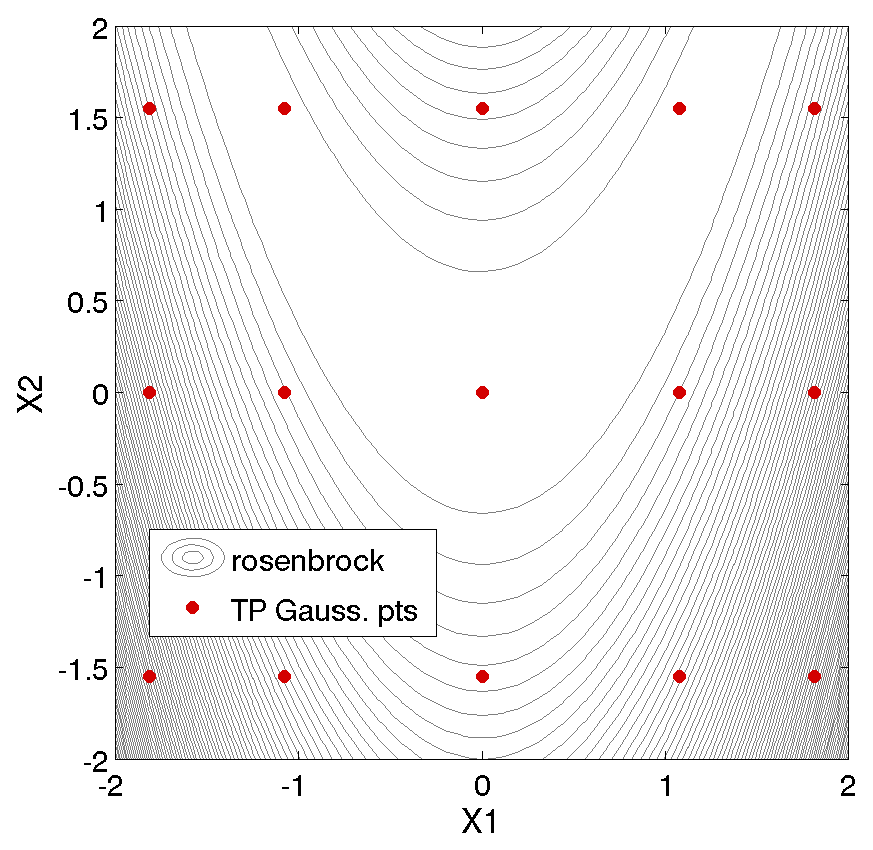
\includegraphics[height=2.5in]{images/rosen_pce_pts}
  \caption{Rosenbrock polynomial chaos example: tensor product quadrature points.}
  \label{uq:examples:rosen_pce_points}
\end{figure}

Once the expansion coefficients have been calculated, some statistics
are available analytically and others must be evaluated numerically.
For the numerical portion, the input file specifies the use of 10000
samples, which will be evaluated on the expansion to compute the CDF
probabilities. In Figure~\ref{uq:examples:pce_out}, excerpts from the
results summary are presented, where we first see a summary of the PCE
coefficients which exactly reproduce Rosenbrock for a Legendre
polynomial basis. The analytic statistics for mean, standard
deviation, and COV are then presented. For example, the mean is 455.66
and the standard deviation is 606.56. The moments are followed by
global sensitivity indices (Sobol' indices).This example shows that
variable x1 has the largest main effect (0.497) as compared with
variable x2 (0.296) or the interaction between x1 and x2 (0.206).
After the global sensitivity indices, the local sensitivities are
presented, evaluated at the mean values.  Finally, we see the
numerical results for the CDF probabilities based on 10000 samples
performed on the expansion. For example, the probability that the
Rosenbrock function is less than 100 over these two uncertain
variables is 0.342. Note that this is a very similar estimate to what
was obtained using 200 Monte Carlo samples, with fewer true function
evaluations.
\begin{figure}[htbp!]
\centering
\begin{bigbox}
%\begin{footnotesize}
\begin{scriptsize}
\begin{verbatim}
Polynomial Chaos coefficients for response_fn_1:
        coefficient   u1   u2
        ----------- ---- ----
   4.5566666667e+02   P0   P0
  -4.0000000000e+00   P1   P0
   9.1695238095e+02   P2   P0
  -9.9475983006e-14   P3   P0
   3.6571428571e+02   P4   P0
  -5.3333333333e+02   P0   P1
  -3.9968028887e-14   P1   P1
  -1.0666666667e+03   P2   P1
  -3.3573144265e-13   P3   P1
   1.2829737273e-12   P4   P1
   2.6666666667e+02   P0   P2
   2.2648549702e-13   P1   P2
   4.8849813084e-13   P2   P2
   2.8754776338e-13   P3   P2
  -2.8477220582e-13   P4   P2
-------------------------------------------------------------------
Statistics derived analytically from polynomial expansion:

Moment-based statistics for each response function:
                            Mean           Std Dev          Skewness          Kurtosis
response_fn_1
  expansion:    4.5566666667e+02  6.0656024184e+02
  numerical:    4.5566666667e+02  6.0656024184e+02  1.9633285271e+00  3.3633861456e+00

Covariance among response functions:
[[  3.6791532698e+05 ]] 

Local sensitivities for each response function evaluated at uncertain variable means:
response_fn_1:
 [ -2.0000000000e+00  2.4055757386e-13 ] 

Global sensitivity indices for each response function:
response_fn_1 Sobol indices:
                                  Main             Total
                      4.9746891383e-01  7.0363551328e-01 x1
                      2.9636448672e-01  5.0253108617e-01 x2
                           Interaction
                      2.0616659946e-01 x1 x2 

Statistics based on 10000 samples performed on polynomial expansion:

Probability Density Function (PDF) histograms for each response function:
PDF for response_fn_1:
          Bin Lower          Bin Upper      Density Value
          ---------          ---------      -------------
   6.8311107124e-03   1.0000000000e-01   2.0393073423e-02
   1.0000000000e-01   1.0000000000e+00   1.3000000000e-02
   1.0000000000e+00   5.0000000000e+01   4.7000000000e-03
   5.0000000000e+01   1.0000000000e+02   1.9680000000e-03
   1.0000000000e+02   5.0000000000e+02   9.2150000000e-04
   5.0000000000e+02   1.0000000000e+03   2.8300000000e-04
   1.0000000000e+03   3.5755437782e+03   5.7308286215e-05

Level mappings for each response function:
Cumulative Distribution Function (CDF) for response_fn_1:
     Response Level  Probability Level  Reliability Index  General Rel Index
     --------------  -----------------  -----------------  -----------------
   1.0000000000e-01   1.9000000000e-03
   1.0000000000e+00   1.3600000000e-02
   5.0000000000e+01   2.4390000000e-01
   1.0000000000e+02   3.4230000000e-01
   5.0000000000e+02   7.1090000000e-01
   1.0000000000e+03   8.5240000000e-01
-------------------------------------------------------------------
\end{verbatim}
\end{scriptsize}
%\end{footnotesize}
\end{bigbox}
\caption{Excerpt of UQ output for polynomial chaos example.}
\label{uq:examples:pce_out}
\end{figure}

\subsubsection{Uncertainty Quantification Example using Stochastic Collocation}
\label{uq:stoch_exp:ex:sc}

%A typical Dakota input file for performing an uncertainty
%quantification using polynomial chaos expansions is shown in
%Section~\ref{uq:stoch_exp:ex:pce}, which illustrates PCE defined from an
%anisotropic tensor-product quadrature grid. The uncertain variables
%are uniforms, so the expansion is built using classical Legendre
%polynomials. 

Compared to the previous PCE example, this section presents a more
sophisticated example, where we use stochastic collocation built on an
anisotropic sparse grid defined from numerically-generated orthogonal
polynomials. The uncertain variables are lognormal in this example and
the orthogonal polynomials are generated from Gauss-Wigert recursion
coefficients~\cite{simpson_gw} in combination with the Golub-Welsch
procedure~\cite{GolubWelsch69}.  The input file is shown in
Figure~\ref{uq:figure11}.  Note that the dimension preference of
$(2,1)$ is inverted to define a $\gamma$ weighting vector of $(0.5,1)$
(and $\underline{\gamma}$ of $0.5$) for use in the anisotropic Smolyak
index set constraint (see Smolyak sparse grids section in Stochastic
Expansion Methods chapter in Dakota Theory Manual~\cite{TheoMan}). In
this example, we compute CDF probabilities for six response levels of
Rosenbrock's function. This example requires 19 function evaluations
to calculate the interpolating polynomials in stochastic collocation
and the resulting expansion exactly reproduces Rosenbrock's function.
The placement of the points generated by the sparse grid is shown in
Figure~\ref{uq:figure11b}.

\begin{figure}[htbp!]
  \centering
  \begin{bigbox}
    \begin{small}
      \verbatimtabinput[8]{../../../test/examples-users/rosen_uq_sc.in}
    \end{small}
  \end{bigbox}
\caption{Dakota input file for performing UQ using stochastic collocation --
see \protect\path{dakota/share/dakota/examples/users/rosen_uq_sc.in} }
\label{uq:figure11}
\end{figure}

\begin{figure}[htbp!]
  \centering
  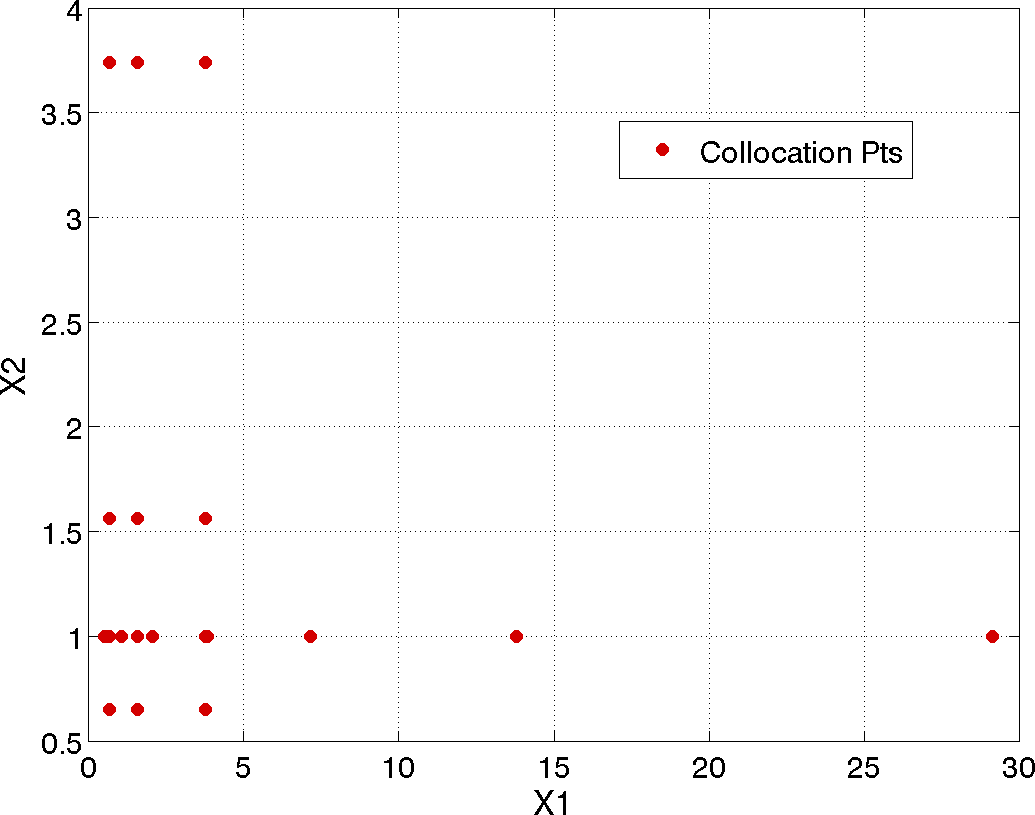
\includegraphics[height=2.5in]{images/rosen_sc_pts}
  \caption{Rosenbrock stochastic collocation example: sparse grid points.}
  \label{uq:figure11b}
\end{figure}

Once the expansion coefficients have been calculated, some statistics
are available analytically and others must be evaluated numerically.
For the numerical portion, the input file specifies the use of 10000
samples, which will be evaluated on the expansion to compute the CDF
probabilities. In Figure~\ref{uq:figure12}, excerpts from the results
summary are presented. We first see the moment statistics for mean,
standard deviation, skewness, and kurtosis computed by numerical
integration (see Analytic moments section in Stochastic Expansion
Methods chapter in Dakota Theory Manual~\cite{TheoMan}), where the
numerical row corresponds to integration using the original response
values and the expansion row corresponds to integration using values
from the interpolant. The response covariance (collapsing to a single
variance value for one response function) and global sensitivity
indices (Sobol' indices) are presented next. This example shows that
variable x1 has the largest main effect (0.99) as compared with
variable x2 (0.0007) or the interaction between x1 and x2 (0.005).
%After the global sensitivity indices, the local, analytic random 
%variable sensitivities are presented, as computed from
%Eqs.~\ref{eq:dR_dx}-\ref{eq:dR_dxi_sc}, evaluated at the mean values.
Finally, we see the numerical results for the CDF probabilities based
on 10000 samples performed on the expansion. For example, the probability 
that the Rosenbrock function is less than 100 is 0.7233. Note that these 
results are significantly different than the ones presented in 
Section~\ref{uq:stoch_exp:ex:pce} because of 
the different assumptions about the inputs: uniform[-2,2] versus
lognormals with means of 1.0 and standard deviations of 0.5. 
\begin{figure}[htbp!]
\centering
\begin{bigbox}
\begin{footnotesize}
\begin{verbatim}
Statistics derived analytically from polynomial expansion:

Moment-based statistics for each response function:
                            Mean           Std Dev          Skewness          Kurtosis
response_fn_1
  expansion:    2.5671972656e+02  2.0484189184e+03  2.7419241630e+02  1.9594567379e+06
  numerical:    2.5671972656e+02  2.0484189184e+03  2.7419241630e+02  1.9594567379e+06

Covariance among response functions:
[[  4.1960200651e+06 ]] 

Global sensitivity indices for each response function:
response_fn_1 Sobol indices:
                                  Main             Total
                      9.9391978710e-01  9.9928724777e-01 x1
                      7.1275222945e-04  6.0802128961e-03 x2
                           Interaction
                      5.3674606667e-03 x1 x2 

Statistics based on 10000 samples performed on polynomial expansion:

Level mappings for each response function:
Cumulative Distribution Function (CDF) for response_fn_1:
     Response Level  Probability Level  Reliability Index  General Rel Index
     --------------  -----------------  -----------------  -----------------
   1.0000000000e-01   1.8100000000e-02
   1.0000000000e+00   8.7800000000e-02
   5.0000000000e+01   5.8410000000e-01
   1.0000000000e+02   7.2330000000e-01
   5.0000000000e+02   9.2010000000e-01
   1.0000000000e+03   9.5660000000e-01
\end{verbatim}
\end{footnotesize}
\end{bigbox}
\caption{Excerpt of UQ output for stochastic collocation example.}
\label{uq:figure12}
\end{figure}

\section{Importance Sampling Methods}\label{uq:importance}

Importance sampling is a method that allows one to estimate statistical
quantities such as failure probabilities (e.g. the probability that
a response quantity will exceed a threshold or fall below a threshold value)
in a way that is more efficient than Monte Carlo sampling. The core idea
in importance sampling is that one generates samples that preferentially
samples important regions in the space (e.g. in or near the failure region
or user-defined region of interest), and then appropriately weights
the samples to obtain an unbiased estimate of the failure probability
~\cite{Srinivasan2002}.
In importance sampling, the samples are generated from a density which is
called the importance density:  it is not the original probability density
of the input distributions. The importance density should be centered near the
failure region of interest. For black-box simulations such as those commonly
interfaced with Dakota, it is difficult to specify the importance density a priori:
the user often does not know where the failure region lies, especially in a high-dimensional
space.~\cite{Swiler2010}

More formally, we define the objective of importance sampling as calculating the probability, $P$, that the output will exceed a threshold level. This is a failure 
probability, where the failure probability is defined as some scalar function, 
$y\left(\textbf{X}\right)$, exceeding a threshold, $T$, 
where the inputs, $\textbf{X}$, are randomly distributed with density, $\rho\left(\textbf{X}\right)$. 
When evaluating $y\left(\textbf{X}\right)$ is sufficiently expensive or $P$ is sufficiently small, Monte Carlo (MC) sampling methods to estimate $P$ will be infeasible due to the large number of function evaluations required
for a specified accuracy. 

The probability of failure can be thought of as the mean rate of occurrence
of failure. The Monte Carlo (MC) estimate of $P$ is therefore the sample
mean of the indicator function, $I\left(\textbf{X}\right)$,
\begin{equation}
P_{MC}=\frac{1}{N}\sum_{i=1}^{N}I\left(\mathbf{X_i}\right)\ \ \textbf{X}\sim \rho\left(\textbf{X}\right),
\label{mc_ind}
\end{equation}
where $N$ samples, $\mathbf{X_i}$, are drawn from
$\rho\left(\textbf{X}\right)$,
and the indicator function $I\left(\textbf{X}\right)$
is 1 if failure occurs and zero otherwise.

Importance sampling draws samples from the importance density 
$\rho'\left(\textbf{X}\right)$ and scales the sample mean by the importance density:
\begin{equation}
P_{IS}=\frac{1}{N}\sum_{i=1}^N \left(I\left(\mathbf{X_i}\right)\frac{\rho\left(\mathbf{X_i}\right)}{\rho'\left(\mathbf{X_i}\right)}\right)\ \ \textbf{X}\sim\rho'\left(\textbf{X}\right).\label{eqn:ispfail}
\end{equation}
This reduces the asymptotic error variance from:
\begin{equation}
\sigma_{err_{MC}}^2=\frac{{\rm E}\left[\left(I\left(\textbf{X}\right)-P\right)^2\right]}{N}
\end{equation}
to
\begin{equation}
\sigma_{err_{IS}}^2=\frac{{\rm E}\left[\left(I\left(\textbf{X}\right)\frac{\rho\left(\textbf{X}\right)}{\rho'\left(\textbf{X}\right)}
-P\right)^2\right]}{N}.
\label{eqn:iserrorvar}
\end{equation}
Inspection of Eq. ~\ref{eqn:iserrorvar} reveals $\sigma_{err_{IS}}^2=0$ if
$\rho'\left(\textbf{X}\right)$ equals the ideal importance density
$\rho^*\left(\textbf{X}\right)$,
\begin{equation}
\rho^*\left(\textbf{X}\right)=\frac{I\left(\textbf{X}\right)\rho\left(\textbf{X}\right)}{P}.\end{equation}
 
However, $\rho^*\left(\textbf{X}\right)$ is unknown a priori because
$I\left(\textbf{X}\right)$ is only known where it has been evaluated. 
Therefore, the required $P$ in the denominator is also unknown:  this is what we are trying to estimate.
 
If importance sampling is to be effective, the practitioner must be able to
choose a good $\rho'\left(\textbf{X}\right)$ without already knowing
$I\left(\textbf{X}\right)$ everywhere. 
There is a danger: a poor choice for $\rho'\left(\textbf{X}\right)$ can put most of the samples in
unimportant regions and make $\sigma_{err_{IS}}^2$ much greater than
$\sigma_{err_{MC}}^2$.
In particular, importance sampling can be challenging for very low probability events in high-dimensional spaces where
the output $y$ is calculated by a simulation. In these cases, usually one
does not know anything a priori about where the failure region exists
in input space. 
We have developed two importance sampling approaches which do not
rely on the user explicitly specifying an importance density.

\subsection{Importance Sampling Method based on Reliability Approach}\label{uq:importance_rel}
The first method is based on ideas in reliability modeling ~\ref{uq:reliability:local}.
An initial Latin Hypercube sampling is performed to generate an initial set of samples.
These initial samples are augmented with samples from an importance density as follows:
The variables are transformed to standard normal space. In the transformed space,
the importance density is a set of normal densities centered around points which
are in the failure region. Note that this is similar in spirit to the reliability
methods, in which importance sampling is centered around a Most Probable Point (MPP).
In the case of the LHS samples, the importance sampling density will simply by
a mixture of normal distributions centered around points in the failure region.

This method is specified by the keyword \texttt{importance\_sampling}.
The options for importance sampling are as follows:  \texttt{import} 
centers a sampling
density at one of the initial LHS samples identified in the failure region.
It then generates the importance samples, weights them by their probability of occurence
given the original density, and calculates the required probability (CDF or CCDF level).
\texttt{adapt\_import} is the same as \texttt{import} but is performed iteratively until the
failure probability estimate converges.
\texttt{mm\_adapt\_import} starts with all of the samples located in the failure region
to build a multimodal sampling density. First, it uses a small number of samples around
each of the initial samples in the failure region. Note that these samples
are allocated to the different points based on their relative probabilities of occurrence:
more probable points get more samples. This early part of the approach is done to 
search for ``representative'' points. Once these are located, the multimodal sampling density is set and then the multi-modal adaptive method proceeds similarly to the 
adaptive method (sample until convergence).
 
\subsection{Gaussian Process Adaptive Importance Sampling Method}\label{uq:gpais}
The second importance sampling method in Dakota is the one we recommend,
at least for problems that have a relatively small number of input variables (e.g.
less than 10). This method, Gaussian Process Adaptive Importance Sampling,
is outlined in the paper ~\cite{Dalbey2014}.
This method  starts with an initial set of LHS samples and adds samples one at a time, 
with the goal of adaptively improving the estimate of the ideal importance density
during the process. The approach uses a mixture of component densities. An
iterative process is used
to construct the sequence of improving component densities. At each
iteration, a Gaussian process (GP) surrogate is used to help identify areas
in the space where failure is likely to occur. The GPs are not used to
directly calculate the failure probability; they are only used to approximate
the importance density. Thus, the Gaussian process adaptive importance
sampling algorithm overcomes limitations involving using a potentially
inaccurate surrogate model directly in importance sampling calculations.

This method is specified with the keyword \texttt{gpais}. There are three 
main controls which govern the behavior of the algorithm. 
\texttt{samples} specifies the initial number of Latin Hypercube samples 
which are used to create the initial Gaussian process surrogate. 
\texttt{emulator\_samples} specifies the number of samples taken on the 
latest Gaussian process model each iteration of the algorithm. 
These samples are used in the construction of the next importance 
sampling density. The default is 10,000 samples. The third control 
is \texttt{max\_iterations}, which controls the number of iterations 
of the algorithm. Each iteration, one additional sample of the ``true'' 
simulation is taken. Thus, if \texttt{samples} were set at 100 and 
\texttt{max\_iterations} were set to 200, there would be a total of 
300 function evaluations of the simulator model taken. 

\section{Adaptive Sampling Methods}\label{uq:adaptive}
The goal in performing adaptive sampling is to construct a surrogate model that
can be used as an accurate predictor to some expensive simulation, thus it is
to one's advantage to build a surrogate that minimizes the error over the entire
domain of interest using as little data as possible from the expensive
simulation. The adaptive part alludes to the fact that the surrogate will be
refined by focusing samples of the expensive simulation on particular areas of
interest rather than rely on random selection or standard space-filling
techniques. 

\subsection{Adaptive sampling based on surrogates}\label{uq:adaptive:surrogate}

At a high-level, the adaptive sampling pipeline is a four-step process:
\begin{enumerate}
\item Evaluate the expensive simulation (referred to as the true model) at
initial sample points
\item Fit/refit a surrogate model
\item Create a candidate set and score based on information from surrogate
\item Select a candidate point to evaluate the true model and Repeat 2-4
\end{enumerate}

In terms of the Dakota implementation, the adaptive sampling method 
currently uses Latin Hypercube sampling (LHS) to generate the initial 
points in Step 1 above. For Step 2, we use a Gaussian process model. 
The user can specify the scoring metric used to select the 
next point (or points) to evaluate and add to the set. 
We have investigated several scoring metrics with which to evaluate 
candidate points for Step 3. There are some classical ones such as distance 
(e.g. add a point which maximizes the minimum distance to all of 
the existing points). This distance metric tends to generate 
points that are space-filling. We have investigated several 
methods that involve interesting topological features of the 
space (e.g. points that are near saddle points). These are 
an area of active investigation but are not currently included 
in Dakota. The fitness metrics for scoring 
candidate points currently include: 
\begin{description}
\item[Predicted Variance]
First introduced in \cite{MacKay} and later
used in \cite{Seo}, this method uses the predicted
variance of the Gaussian process surrogate as the score of a candidate 
point. Thus, the adaptively chosen points will be in areas of highest 
uncertainty according to the Gaussian process model.
\item[Distance]
A candidate's score is the Euclidean distance in domain space between the
candidate and its nearest neighbor in the set of points already evaluated on the
true model. Therefore, the most undersampled area of the domain will always be
selected. The adaptivity of this method could be brought to question as it would
chose the exact same points regardless of the surrogate model used. However, it
is useful to use to compare other adaptive metrics to one that relies purely on
space-filling in an equivalent context.
\item[Gradient]
%DPM: PROBABLY WANT TO CHANGE THE NAME OF THIS METRIC
Similar to the above metric, a candidate's nearest neighbor is determined as in
the distance metric, only now the score is the absolute value of the difference
in range space of the two points. The range space values used are predicted
from the surrogate model. Though this method is called the gradient metric, it
actually does not take into account how close the candidate and its neighbor are
in domain space. This method attempts to evenly fill the range space of the
surrogate.
\end{description}

Note that in our approach, a Latin Hypercube sample is generated (a new one, 
different from the initial sample) and the surrogate model is evaluated 
at this points. These are the ``candidate points'' that are then evaluated 
according to the fitness metric outlined above. The number of candidates used 
in practice should be high enough to fill most
of the input domain: we recommend at least hundreds of points for a low-
dimensional problem. 
All of the candidates (samples on the emulator) are 
given a score and then the highest-scoring candidate is selected to be evaluated
on the true model. 

The adaptive sampling method also can generate batches of points 
to add at a time. With batch or  multi-point 
selection, the true model can be evaluated in parallel and thus
increase throughput before refitting our surrogate model. This proposes a new
challenge as the problem of choosing a single point and choosing multiple points
off a surrogate are fundamentally different. Selecting the $n$ best scoring
candidates is more than likely to generate a set of points clustered in one
area which will not be conducive to adapting the surrogate.
We have implemented several strategies for batch selection of points: 
\begin{description}
\item[\bf Naive Selection]  
This strategy will select the $n$ highest scoring candidates regardless of their
position. This tends to group an entire round of points in the same area.
\item[\bf Distance Penalized Re-weighted Scoring] 
In this strategy, the highest 
scoring candidate is selected and then all
remaining candidates are re-scored with a distance penalization factor added in
to the score. Only points selected within a round are used for the distance
penalization. The factor is the same as used in the distance penalization
 scoring metrics from \cite{Maljovec}. First, compute all of the minimum
distances from each remaining candidate to the selected candidates. Then,
determine the median value of these distances. If the smallest distance, $d$,
between a point and the selected set is less than the computed median distance
its score is unaltered, otherwise the score is multiplied by a value $\rho$
determined by the following equation:
\begin{equation}
\rho = 1.5*d - 0.5*d^3
\end{equation}
\item[\bf Topological Maxima of Scoring Function]  
In this strategy we look at the topology of the scoring function and select the
$n$ highest maxima in the topology. To determine local maxima, we construct the
approximate Morse-Smale complex. If the number of local maxima is less than $n$,
 we revert to the distance strategy above. As a further extension, one may
want to filter low-persistence maxima, but to keep the framework general, we
chose to omit this feature as defining a threshold for what deems a critical
point as "low persistence" can vary drastically from problem to problem.
\item[\bf Constant Liar]  
We adapt the constant liar strategy presented in \cite{Ginsbourger} with the
scoring metrics. The strategy first selects
the highest scoring candidate, and then refits the surrogate using a ``lie'' value
at the point selected and repeating until $n$ points have been selected
whereupon the lie values are removed from the surrogate and the selected points
are evaluated on the true model and the surrogate is refit with these values.
\end{description}

The adaptive sampling method is specified by the method keyword 
\texttt{adaptive\_sampling}. There are many controls, including 
the number of candidate samples to investigate each iteration 
(\texttt{emulator\_samples}), the fitness metric used in scoring 
candidates (\texttt{fitness\_metric}), and the number of iterations 
to perform the adaptive sampling (\texttt{max\_iterations}). 
For batch selection of points, one specifies a \texttt{batch\_selection} 
strategy and a \texttt{batch\_size}. 
The details of the specification are provided in the Dakota 
reference manual. 

\subsection{Adaptive sampling based on dart throwing}\label{uq:adaptive:darts}
\texttt{pof\_darts} is a novel method for estimating the tail probability
(Probability of Failure) based on random sphere-packing in the uncertain
parameter space. Random points are sequentially sampled from the domain and
consequently surrounded by protecting spheres, with the constraint that each new
sphere center has to be outside all prior spheres~\cite{ebeida2016pof}. The
radius of each sphere is chosen such that the entire sphere lies either in the
failure or the non-failure region. This radius depends of the function
evaluation at the disk center, the failure threshold and an estimate of the
function gradient at the disk center. After exhausting the sampling budget
specified by \texttt{build\_samples}, which is the number of spheres per failure
threshold, the domain is decomposed into two regions.  These regions correspond
to failure and non-failure categories, each represented by the union of the
spheres of each type. The volume of the union of failure spheres gives a lower
bound on the required estimate of the probability of failure, while the volume
of the union of the non-failure spheres subtracted from the volume of the domain
gives an upper estimate. After all the spheres are constructed, we construct a
surrogate model, specified via a \texttt{model\_pointer}, and sample the
surrogate model extensively to estimate the probability of failure for each
threshold. 

\texttt{pof\_darts} handles multiple response functions and allows each to have
multiple failure thresholds. For each failure threshold \texttt{pof\_darts} will
insert a number of spheres specified by the user-input parameter "samples".
However, estimating the probability of failure for each failure threshold would
utilize the total number of disks sampled for all failure thresholds. For each
failure threshold, the sphere radii changes to generate the right spatial
decomposition. The POF-Darts method is specified by the method keyword
\texttt{pof\_darts}. The sample budget is specified by \texttt{build\_samples}.
By default, the method employs a local approach to estimate the Lipschitz
constant per sphere.
%The method can generally support local or global approaches to estimate the
%Lipschitz constant per sphere, given by (\texttt{lipschitz local} or
%\texttt{lipschitz global}). However, only the local approach is currently
%supported and is the default if not specified by the user.

The surrogate model used by the \texttt{pof\_darts} method for extensive
sampling is specified using a \texttt{model\_pointer}, and its parameters are
therefore defined in that model. It can typically be any global surrogate in
Dakota (e.g., Gaussian process, polynomial chaos expansion, polynomial
regression, etc). POF-Darts can also use piecewise-decomposed surrogates which
build local pieces of the surrogate over different domain patches. The piecewise
decomposition option is a new capability added to Dakota to help construct
surrogates in high-dimensional spaces, using known function evaluations as well
as gradient and Hessian information, if available. The piecewise decomposition
option is declared using the keyword \texttt{domain\_decomp} and currently
supports polynomial, Gaussian Process (GP), and Radial Basis Functions (RBF)
surroagte models only. For example: a polynomial regression global surrogate is
specified with \texttt{model polynomial}, its order is selected using
\texttt{surrogate\_order}, and the piecewise decomposition option is specified
with \texttt{domain\_decomp}. The \texttt{domain\_decomp} option is parametrized
by a \texttt{cell\_type} set by default to Voronoi cells, an optional number of
\texttt{support\_layers}, and an optional \texttt{discontinuity\_detection}
capability. See~\ref{models:surf:piecewise_decomp} for more details.

\section{Epistemic Nondeterministic Methods}\label{uq:epistemic}

Uncertainty quantification is often used as part of the risk
assessment of performance, reliability, and safety of engineered
systems. Increasingly, uncertainty is separated into two categories
for analysis purposes: aleatory and epistemic
uncertainty~\cite{Obe03,Hel07}. Aleatory uncertainty is also referred to as
variability, irreducible or inherent uncertainty, or uncertainty due
to chance. Examples of aleatory uncertainty include the height of
individuals in a population, or the temperature in a processing
environment. Aleatory uncertainty is usually modeled with probability
distributions, and sampling methods such as Latin Hypercube sampling
in Dakota can be used to model aleatory uncertainty. In contrast,
epistemic uncertainty refers to lack of knowledge or lack of
information about a particular aspect of the simulation model,
including the system and environment being modeled. An increase in
knowledge or information relating to epistemic uncertainty will lead
to a reduction in the predicted uncertainty of the system response or
performance. For epistemic uncertain variables, typically one does not
know enough to specify a probability distribution on a variable.
Epistemic uncertainty is referred to as subjective, reducible, or lack
of knowledge uncertainty. Examples of epistemic uncertainty include
little or no experimental data for a fixed but unknown physical
parameter, incomplete understanding of complex physical phenomena,
uncertainty about the correct model form to use, etc.

There are many approaches which have been developed to model epistemic
uncertainty, including fuzzy set theory, possibility theory, and
evidence theory. It is also possible to use simple interval analysis in 
an epistemic context. Interval analysis and evidence theory are 
described in more detail below.

\subsection{Interval Methods for Epistemic Analysis}\label{uq:interval}

In interval analysis, one assumes that nothing is known about 
an epistemic uncertain variable except that its value lies 
somewhere within an interval. In this situation, it is NOT 
assumed that the value has a uniform probability of occuring 
within the interval. Instead, the interpretation is that 
any value within the interval is a possible value or a potential 
realization of that variable. In interval analysis, the 
uncertainty quantification problem is one of determining the 
resulting bounds on the output (defining the output interval) 
given interval bounds on the inputs. Again, any output response 
that falls within the output interval is a possible output 
with no frequency information assigned to it.

We have the capability to perform interval analysis using either
\dakotakw{global_interval_est} or \dakotakw{local_interval_est}.  In
the global approach, one uses either a global optimization method or a
sampling method to assess the bounds.  \texttt{global\_interval\_est}
allows the user to specify either \texttt{lhs}, which performs Latin
Hypercube Sampling and takes the minimum and maximum of the samples as
the bounds (no optimization is performed) or \texttt{ego}. In the case
of \texttt{ego}, the efficient global optimization method is used to
calculate bounds. The ego method is described in
Section~\ref{opt:methods:gradientfree:global}.  If the problem is
amenable to local optimization methods (e.g. can provide derivatives
or use finite difference method to calculate derivatives), then one
can use local methods to calculate these
bounds. \texttt{local\_interval\_est} allows the user to specify
either \texttt{sqp} which is sequential quadratic programming, or
\texttt{nip} which is a nonlinear interior point method.

Note that when performing interval analysis, it is necessary to define
interval uncertain variables as described in
Section~\ref{variables:uncertain}. For interval analysis, one must
define only one interval per input variable, in contrast with
Dempster-Shafer evidence theory, where an input can have several
possible intervals. Interval analysis can be considered a special
case of Dempster-Shafer evidence theory where each input is defined by
one input interval with a basic probability assignment of one. In
Dakota, however, the methods are separate and semantic differences
exist in the output presentation. If you are performing a pure
interval analysis, we recommend using either
\texttt{global\_interval\_est} or \texttt{local\_interval\_est}
instead of \texttt{global\_evidence} or \texttt{local\_evidence}, for
reasons of simplicity. %An example of interval estimation is found in
%the \path{dakota/share/dakota/examples/users/cantilever_uq_global_interval.in},
%and also in Section~\ref{uq:examples:interval}.

%Note that we have kept separate implementations of interval analysis and
%Dempster-Shafer evidence theory because our users often want to couple
%interval analysis on an ``outer loop'' with an aleatory, probabilistic
%analysis on an ``inner loop'' for nested, second-order probability
%calculations. See Section~\ref{adv_models:mixed_uq} for additional
%details on these nested approaches.
These interval methods can also be used as the outer loop within an
interval-valued probability analysis for propagating mixed aleatory
and epistemic uncertainty -- refer to
Section~\ref{adv_models:mixed_uq:ivp} for additional details.

%\subsubsection{Interval Analysis for Cantilever}\label{uq:examples:interval}

%Interval analysis is often used to model epistemic uncertainty. 
%In interval analysis, the 
%uncertainty quantification problem is one of determining the 
%resulting bounds on the output (defining the output interval) 
%given interval bounds on the inputs. 

%We can do interval analysis using either
%\texttt{global\_interval\_est} or \texttt{local\_interval\_est}.
%In the global approach, one uses either a global optimization 
%method or a sampling method to assess the bounds, whereas the 
%local method uses gradient information in a derivative-based 
%optimization approach. 
 
An example of interval estimation 
is shown in Figure~\ref{uq:examples:interval_input}, with example results in 
Figure~\ref{uq:examples:interval_out}. This example is a demonstration 
of calculating interval bounds for three outputs of the cantilever beam 
problem. The cantilever beam problem is described in detail in 
Section~\ref{additional:cantilever}. Given input intervals of [1,10] on 
beam width and beam thickness, we can see that the interval estimate of 
beam weight is approximately [1,100].

\begin{figure}[htbp!]
  \centering
  \begin{bigbox}
    \begin{small}
      \verbatimtabinput[8]{../../../test/examples-users/cantilever_uq_global_interval.in}
    \end{small}
  \end{bigbox}
\caption{Dakota input file for performing UQ using interval analysis --
see \protect\path{dakota/share/dakota/examples/users/cantilever_uq_global_interval.in} }
\label{uq:examples:interval_input}
\end{figure}

\begin{figure}[htbp!]
\centering
\begin{bigbox}
\begin{small}
\begin{verbatim}
------------------------------------------------------------------
Min and Max estimated values for each response function:
weight:  Min = 1.0000169352e+00  Max = 9.9999491948e+01
stress:  Min = -9.7749994284e-01  Max = 2.1499428450e+01
displ:  Min = -9.9315672724e-01  Max = 6.7429714485e+01
-----------------------------------------------------------------
\end{verbatim}
\end{small}
\end{bigbox}
\caption{Excerpt of UQ output for interval example.}
\label{uq:examples:interval_out}
\end{figure}


\subsection{Dempster-Shafer Theory of Evidence}\label{uq:dempshaf}

We have chosen to pursue evidence theory at Sandia as a way to model
epistemic uncertainty, in part because evidence theory is a
generalization of probability theory. Evidence theory is also
referred to as Dempster-Shafer theory or the theory of random
sets~\cite{Obe03}. This section focuses on the use of Dempster-Shafer
evidence theory for propagating epistemic uncertainties. When
aleatory uncertainties are also present, we may choose either to
discretize the aleatory probability distributions into sets of
intervals and treat them as well-characterized epistemic variables, or
we may choose to segregate the aleatory uncertainties and treat them
within an inner loop. A nested Dempster-Shafer approach for
propagating mixed aleatory and epistemic uncertainty is described in
Section~\ref{adv_models:mixed_uq:dste}.
%We also use a technique called second-order probability to perform
%uncertainty quantification when there is both epistemic and aleatory
%uncertainty present. Second-order probability is a nested technique
%with two levels of uncertainty quantification. The outer level UQ is
%typically linked to epistemic uncertainties and the inner level UQ is
%commonly associated with aleatory uncertainties. A common approach
%used is to sample possible realizations of epistemic variables in the
%outer loop, then send these to the inner loop for additional sampling
%over the aleatory variables. In this way one generates ``families''
%or ensembles of cumulative distribution functions, where each
%individual CDF is based on aleatory uncertainty, and the ensemble is
%based on epistemic uncertainty. See Section~\ref{adv_models:mixed_uq}
%for more details.

In evidence theory, there are two complementary measures of
uncertainty: belief and plausibility. Together, belief and
plausibility can be thought of as defining lower and upper bounds,
respectively, on probabilities. Belief and plausibility define the
lower and upper limits or intervals on probability values. Typical
plots of cumulative and complementary cumulative belief and
plausibility functions are shown in Figure~\ref{uq:figure15}~\cite{Hel07}.
\begin{figure}[htbp!]
  \centering 
  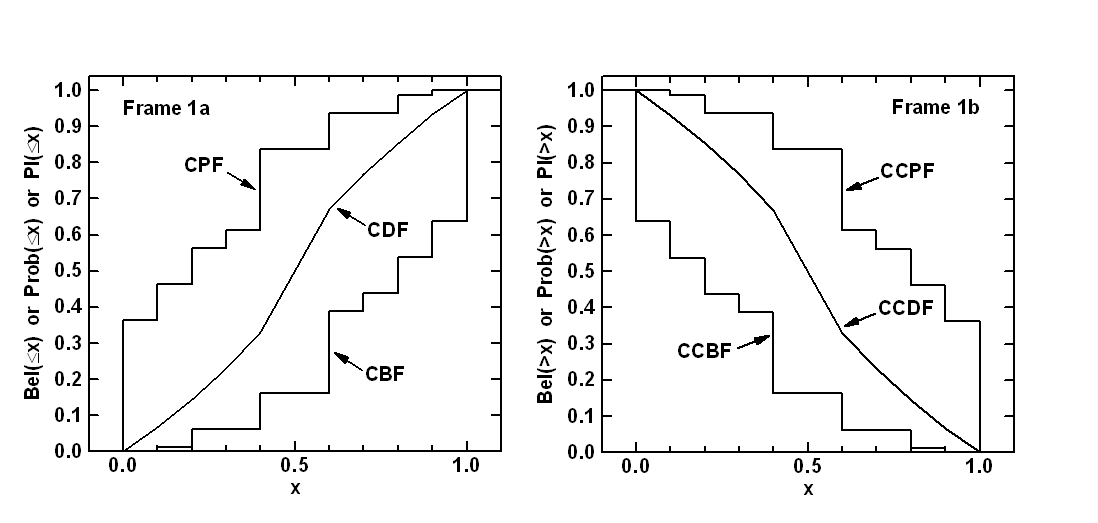
\includegraphics[scale=0.8]{images/belief_plaus} 
  \caption{Example cumulative belief and plausibility distribution functions on left; complementary cumulative belief and plausibility distribution functions on right}
  \label{uq:figure15}
\end{figure}
In evidence theory, it is not possible to specify one probability value.
Instead, there is a range of values that is consistent with the
evidence. The range of values is defined by belief and
plausibility. Note that no statement or claim is made about one value
within an interval being more or less likely than any other value.

In Dempster-Shafer evidence theory, the uncertain input variables are
modeled as sets of intervals. The user assigns a basic probability
assignment (BPA) to each interval, indicating how likely it is that
the uncertain input falls within the interval. The BPAs for a
particular uncertain input variable must sum to one. The intervals
may be overlapping, contiguous, or have gaps. In Dakota, an interval
uncertain variable is specified as \dakotakw{interval_uncertain}. When
one defines an interval type variable in Dakota, it is also necessary
to specify the number of intervals defined for each variable with
\dakotakw{iuv_num_intervals} as well the basic probability assignments
per interval, \dakotakw{iuv_interval_probs}, and the associated bounds
per each interval, \dakotakw{iuv_interval_bounds}. 
Figure~\ref{uq:figure16} shows the input specification for interval
uncertain variables. 
The example has two epistemic uncertain interval variables. 
The first uncertain
variable has three intervals and the second has two. The basic
probability assignments for the first variable are 0.5, 0.1, and 0.4,
while the BPAs for the second variable are 0.7 and 0.3. Note that it
is possible (and often the case) to define an interval uncertain
variable with only ONE interval. This means that you only know that
the possible value of that variable falls within the interval, and the
BPA for that interval would be 1.0. In the case we have shown, the
interval bounds on the first interval for the first variable are 0.6
and 0.9, and the bounds for the second interval for the first variable
are 0.1 to 0.5, etc.

\begin{figure}[htbp!]
  \centering
  \begin{bigbox}
    \begin{small}
      \verbatimtabinput[8]{../../../test/examples-users/textbook_uq_glob_evidence.in}
    \end{small}
  \end{bigbox}
\caption{Dakota input file for UQ example using Evidence Theory --
see \protect\path{dakota/share/dakota/examples/users/textbook_uq_glob_evidence.in} }
\label{uq:figure16}
\end{figure}

Once the intervals, the BPAs, and the interval bounds are defined, 
the user can run an epistemic analysis by specifying the method as 
either \texttt{global\_evidence} or 
\texttt{local\_evidence} in the Dakota input file. 
Both of these methods perform Dempster-Shafer calculations:  
the difference is that the local method uses a local optimization 
algorithm to calculate the interval bounds and the global 
method uses either sampling or a global optimization approach to 
calculate an interval bound. These differences are discussed in 
more detail below. 
The intervals and their associated BPAs are then propagated through
the simulation to obtain cumulative distribution functions on belief
and plausibility. As mentioned above, belief is the lower bound on a
probability estimate that is consistent with the evidence, and
plausibility is the upper bound on a probability estimate that is
consistent with the evidence. 

Figure~\ref{uq:figure17} shows
results for the first response function obtained when running the
example in Figure~\ref{uq:figure16}. In this example, there are 6
output intervals (as a result of the 2 interval input variables with 3
and 2 intervals, respectively). 
The output intervals are ordered to obtain cumulative
bound functions for both belief and plausibility. The
cumulative distribution function is presented for both belief (CBF) and
plausibility (CPF). The CBF value is the cumulative belief
corresponding to a certain output value. For example, the belief that
the output value is less than or equal to 0.2 for response 1 is 0.27, 
and the plausibility that the output is less than
or equal to 0.2 is 1 for response 1. The belief that the 
output value is less than 0.6217 is 0.75, while the plausbility that 
the output is less than  0.0806 is 0.75. 
The CBF and CPF may be plotted on a graph and
interpreted as bounding the cumulative distribution
function (CDF), which is the probability that the output is less than or equal
to a certain value. The interval bounds on probability values show
the value of epistemic uncertainty analysis: the intervals are usually
much larger than expected, giving one a truer picture of the total
output uncertainty caused by lack of knowledge or information about
the epistemic input quantities.

\begin{figure}[htbp!]
\centering
\begin{bigbox}
\begin{small}
\begin{verbatim}
Belief and Plausibility for each response function:
Cumulative Belief/Plausibility Functions (CBF/CPF) for response_fn_1:
     Response Level  Belief Prob Level   Plaus Prob Level
     --------------  -----------------   ----------------
   1.0000000000e-03   0.0000000000e+00   0.0000000000e+00
   3.0000000000e-02   0.0000000000e+00   2.7000000000e-01
   2.0000000000e-01   2.7000000000e-01   1.0000000000e+00
   8.0000000000e-01   9.3000000000e-01   1.0000000000e+00
  Probability Level  Belief Resp Level   Plaus Resp Level
  -----------------  -----------------   ----------------
   2.5000000000e-01   2.6187288772e-01   6.2609206069e-02
   5.0000000000e-01   2.9829775860e-01   6.3736734971e-02
   7.5000000000e-01   6.2173551556e-01   8.0596931719e-02
\end{verbatim}
\end{small}
\end{bigbox}
\caption{Results of an Epistemic Uncertainty Quantification using Evidence Theory.}
\label{uq:figure17}
\end{figure}

As in other nondeterministic methods, with \texttt{local\_evidence}
or \texttt{global\_evidence},
one can specify probability levels and response levels. 
If response levels are specified, the belief and plausibility 
function values corresponding to those response levels are calculated 
(see Belief Prob Level and Plaus Prob Level in the tables shown in 
Figure~\ref{uq:figure17}). Similarly, if probability levels are 
specified, these are first interpreted to be belief values, and the 
corresponding response levels are calculated (see Belief Resp Level); 
then they are interpreted to be plausibility values and the 
corresponding response levels are calculated (see Plaus Resp Level in 
the table in Figure~\ref{uq:figure17}). We have recently added the 
capability to support generalized reliability mappings in 
the evidence methods. If the user specifies a generalized 
reliability level, it will be first converted to a probability, 
then interpreted as a belief and plausibility and the corresponding 
response levels will be calculated. Likewise, if response levels 
are specified, the corresponding belief and plausibility values 
will be mapped to bounds on the generalized reliability levels. 

To elaborate on the differences between \texttt{global\_evidence} and
\texttt{local\_evidence}: both of these methods take the
Dempster-Shafer structures specified on the inputs and calculate a
resulting Dempster-Shafer structure on the outputs (e.g. a cumulative
belief and plausibility function).  To calculate the belief and
plausibility measures, it is necessary to calculate the minimum and
maximum of the response function in each ``interval cell
combination.''  For example, in a two variable problem, if the first
variable had three intervals and associated BPAs assigned and the
second variable had two intervals and associated BPAs assigned, there
would be 6 interval cells in total.  In each of these six cells, one
needs to identify a minimum and maximum value of the response
function. This is easy to do if the function is monotonic in both
variables, but in general it is not. We offer the capability to use
local optimization methods to calculate these bounds:
\texttt{local\_evidence} allows the user to specify either
\texttt{sqp} which is sequential quadratic programming, or
\texttt{nip} which is a nonlinear interior point method. We also offer
the capability to use global methods to assess these interval cell
bounds. \texttt{global\_evidence} allows the user to specify either
\texttt{lhs}, which performs Latin Hypercube Sampling and takes the
minimum and maximum of the samples within each cell as the bounds (no
optimization is performed) or \texttt{ego}. In the case of
\texttt{ego}, the efficient global optimization method is used to
calculate bounds. The \texttt{ego} method is described in
Section~\ref{opt:methods:gradientfree:global}.  Note that for a
situation with many uncertain variables, each with a fairly
complicated Dempster-Shafer structure described by many intervals,
there will be a huge number of interval calls, and the overall process
of performing Dempster-Shafer analysis will be extremely expensive.
Reference~\cite{Tang10b} provides more details about the
implementation of the optimization methods to perform Dempster-Shafer
calculations, as well as comparisons on test problems.

\section{Bayesian Calibration Methods}\label{uq:bayesian}

In Bayesian calibration a ``prior distribution'' on a parameter is
updated through a Bayesian framework involving experimental data and a
likelihood function.  Bayesian inference theory is best left to other
sources ~\cite{Kenn01} and only a brief summary is given here.  In
Bayesian methods, uncertain parameters are characterized by
probability density functions. These probability density functions
define the permissible parameter values - the support, as well as the
relative plausibility of each permissible parameter value. In the
context of calibration or any inference step, the probability density
function that describes knowledge before the incorporation of data is
called the prior, $f_{\boldsymbol{\Theta}}\left( \boldsymbol{\theta}
\right)$.
 
Note: In Dakota, the prior distribution is characterized by the
properties of the active uncertain variables. Correlated priors are
only supported for unbounded normal, untruncated lognormal, uniform,
exponential, gumbel, frechet, and weibull distributions and require a
probability transformation by specifying
\dakotakw{standardized_space}.

When data are available, the likelihood function describes how well
each parameter value is supported by the data. Bayes
Theorem~\cite{Jaynes}, shown in Equation~\ref{eq:BayesThm}, is used
for inference: to derive the plausible parameter values, based on the
prior probability density and the data $\boldsymbol{d}$. The result is
the posterior probability density function of the parameters
$f_{\boldsymbol{{\Theta |D}}}\left( \boldsymbol{{\theta |d}}
\right)$. It is interpreted the same way as the prior, but includes
the information derived from the data.
 
\begin{equation}
{f_{\boldsymbol{\Theta |D}}}\left( \boldsymbol{\theta |d} \right) = \frac{{{f_{\boldsymbol{\Theta}}}\left( \boldsymbol{\theta}  \right)\mathcal{L}\left( \boldsymbol{\theta;d} \right)}}{{{f_{\boldsymbol{D}}}\left( \boldsymbol{d} \right)}}. \label{eq:BayesThm}
\end{equation}


%\begin{equation}
%  \label{eqn:BayesThm}
%  {f_{\Theta |D}}\left( {\theta |d} \right) = \frac{{{f_\Theta }\left( \theta  \right)\mathcal{L}\left( {\theta ;d} \right)}}{{{f_D}\left( d \right)}}
%\end{equation}

The likelihood function is used to describe how well a model's
predictions are supported by the data.  The likelihood function can be
written generally as:
\begin{equation*}
  \mathcal{L}\left(\boldsymbol{{\theta ;d}} \right) =  \mathcal{F}(q(\boldsymbol{\theta)} -\boldsymbol{d}),
\end{equation*}
where $\boldsymbol{\theta}$ are the parameters of model quantity of
interest $q$.  The form of the function $\mathcal{F}$ can greatly
influence the results.  The specific likelihood function used in
Dakota is based on Gaussian probability density functions. This means
that we assume the difference between the model quantity
(e.g. quantity of interest returned from a computer simulation) and
the experimental observations are Gaussian:
\begin{equation}\label{eq:model}
d_i = q_i(\boldsymbol{\theta}) + \epsilon_i,
\end{equation}
where $\epsilon_i$ is a random variable that can encompass both
measurement errors on $d_i$ and modeling errors associated with the
simulation quantity of interest $q_i$, for each of $n$ observations.

If we assume that all experiments and observations are independent,
then the probabilistic model defined by Eq.~(\ref{eq:model}) results
in a likelihood function for $\boldsymbol{\theta}$ that is the product
of $n$ normal probability density functions:
%as shown in Equation~\ref{eqn:Likelihood}.
\begin{equation}\label{eqn:Likelihood}  
\mathcal{L}(\boldsymbol{{\theta};d}) = \prod_{i=1}^n
\frac{1}{\sigma_d \sqrt{2\pi}} \exp
\left[ - \frac{\left(d_i-q_i(\boldsymbol{{\theta}})\right)^2}{2{\sigma_d}^2} \right],
%\mathcal{L}\left( {{\theta};d} \right) = \prod\limits_{i = 1}^n {\frac{1}{{\sigma \sqrt {2\pi } }}  \exp \left[  - \frac{\left(d_i - \mathcal{M}({\theta})\right)^2}{2\sigma^2} \right]
\end{equation}
where ${\sigma_d}^2$ refers to the measurement error of the data,
assumed constant across all data observations in this case.

We also support the more general case of a full covariance matrix,
$\boldsymbol{\Sigma_d}$, that specifies the covariance between each
observation $i$ and $j$.  In this case, the likelihood is commonly
written in log form, where the log-likelihood
is: %given in Equation~\ref{eqn:LogLikelihood}.
\begin{equation}\label{eqn:LogLikelihood}  
\log{\mathcal{L}(\boldsymbol{{\theta};d})} \propto % =-0.5 {R}^{T} {\Sigma_d}^{-1} {R}
-\frac{1}{2} \boldsymbol{r}^T \boldsymbol{\Sigma_d}^{-1} \boldsymbol{r},
\end{equation}
where $\boldsymbol{r}$ is the vector of residuals between the data
points and the model quantity of interest,
$q(\boldsymbol{\theta})-\boldsymbol{d}$.

Dakota admits four \texttt{experiment\_variance\_type} options to specify the
measurement error covariance: \texttt{none} for no measurement error
specified (in this case, the variance is assumed to be one),
\texttt{scalar} where a constant value ${\sigma_d}^2$ is given for all
observations, \texttt{diagonal} where a value is specified for the
diagonal elements of the covariance matrix $\boldsymbol{\Sigma_d}$
meaning that each observation has its own measurement error but there
are no cross terms, and \texttt{matrix} where the full covariance
matrix $\boldsymbol{\Sigma_d}$ is specified.  The \texttt{diagonal}
and \texttt{matrix} terms are only available for field response data.
In contrast to earlier versions of Dakota, all measurement error
variance should be specified with units of variance/covariance, not
standard deviation.

Markov Chain Monte Carlo (MCMC) is the prototypical method used to
estimate posterior parameter densities, given the observational data
and the priors. There are many references that describe the basic
algorithm~\cite{Gilks} and this is an active research area.  MCMC
algorithms may require hundreds of thousands of steps to converge,
depending on dimensionality, response nonlinearity, and the desired
set of posterior statistics.  Since each iteration involves an
evaluation of the model to obtain $q(\boldsymbol{\theta})$, surrogate
models of expensive simulations are often employed to make the MCMC
process tractable.
 
Dakota offers five approaches for Bayesian calibration: QUESO, DREAM,
GPMSA, MUQ, and WASABI.  They are specified with the
\texttt{bayes\_calibration} keyword in combination with the
\texttt{queso}, \texttt{dream}, \texttt{gpmsa}, \texttt{muq}, or \texttt{wasabi}
selections, respectively.  The QUESO and GPMSA methods use components
from the QUESO library (Quantification of Uncertainty for Estimation,
Simulation, and Optimization) developed at The University of Texas at
Austin.  It implements the Delayed Rejection and Adaptive
Metropolis~\cite{Haario} (DRAM) algorithm, among others.  Algorithm
variants selectively combine the delayed rejection and adaptive
elements.  The QUESO/GPMSA capability is based on the GPMSA Matlab
toolbox developed at Los Alamos National Laboratory and uses tightly
integrated Gaussian process models during calibration.  The Dakota
implementation of QUES0/GPMSA is in a prototype stage.  DREAM uses an
implementation of DiffeRential Evolution Adaptive Metropolis developed
by John Burkardt.  The DREAM approach runs concurrent chains for
global exploration, and automatically tunes the proposal covariance
during the process by a self-adaptive randomized subspace
sampling~\cite{Vrugt}. MUQ uses components from the MIT 
Uncertainty Quantification library and also implements the Delayed Rejection
and Adaptive Metropolis~\cite{Haario} (DRAM) algorithms, among others.
The prototype WASABI method is an MCMC-free Bayesian calibration
approach.  QUESO/DRAM and variants are the most well-developed within
Dakota.

\subsection{QUESO}\label{uq:bayesian:queso}
The QUESO library includes several sampling algorithm variants.  One
can use a standard Metropolis-Hastings algorithm
(\texttt{metropolis\_hastings}), adaptive Metropolis
(\texttt{adaptive\_metropolis}) for adapting the proposal covariance
during the sampling, delayed rejection (\texttt{delayed\_rejection})
for backtracking from sample rejections, the full DRAM (\texttt{dram})
which involves both delayed rejection and adaptive Metropolis, or a
multi-level algorithm (\texttt{multilevel}).  This last option is not
yet production-ready in Dakota. 

With any choice of sampling algorithm, one may manually set the burn in 
period for the MCMC chain with \texttt{burn\_in\_samples}. If a 
\texttt{sub\_sampling\_period} is specified, the MCMC chain is further 
filtered such that only the sample at the beginning of each period is in 
the final MCMC chain. The \texttt{sub\_sampling\_period} should therefore 
be greater than or equal to the correlation length of the samples.

With the QUESO method, one may run the MCMC sampling on the simulation
model directly.  However, if the model is expensive, use of a
surrogate (emulator) model is recommended.  Options include a Gaussian
process, a polynomial chaos expansion, or a stochastic collocation
expansion.

The proposal covariance refers to the covariance structure of a
multivariate normal distribution, which governs sample generation in
the chain.  One may specify \texttt{proposal\_covariance}, followed by
\texttt{prior} (the default), \texttt{values}, \texttt{filename}, or
\texttt{derivatives}.  With the \texttt{prior} setting, the proposal
covariance will be set to the variance of the prior distributions of
the parameters being calibrated.  When specifying the proposal
covariance with input file values or from a separate file, the user
may specify only the diagonals of the covariance matrix or the full
covariance matrix.

The derivatives option will use derivatives from the simulation or
emulator model to form or approximate the Hessian of the misfit
function (the negative log likelihood).  Especially when derivative
information is available inexpensively (e.g. from an emulator), the
derivative-based proposal covariance forms a more accurate proposal
distribution, resulting in lower rejection rates and faster chain
mixing.  When using an emulator, the derivative-based proposal
covariance should be updated periodically using the
\texttt{posterior\_adaptive} specification.  This will add simulation
truth evaluations in areas of high-likelihood to the emulator training
data, thus refining the Hessian.  For more detail about
derivative-based formulations involving the misfit Hessian, refer to
the Theory Manual.

An additional control for QUESO is to perform a logit transformation
(\texttt{logit\_transform}) which performs an internal variable
transformation from bounded domains to unbounded
domains. %in order to reduce sample rejection due to an out-of-bounds condition.
This option can be helpful when regions of high posterior density
exist in the corners of a multi-dimensional bounded domain.  In these
cases, it may be difficult to generate feasible samples from the
proposal density, and transformation to unbounded domains may
greatly reduce sample rejection rates.

The \texttt{pre\_solve} option will perform a deterministic
gradient-based optimization before the MCMC sampling to get a good
starting point for the chain.  This pre-solve seeks to maximize the
log-posterior (the log-likelihood minus the log-prior) to identify the
maximum a posteriori probability point, also called the MAP point.
The Markov Chain will then start at the MAP point, which can
circumvent a lot of initial searching for high posterior probability
points.  The pre-solve option can be used with an emulator or with no
emulator.

Credible and prediction intervals will be calculated if 
\texttt{probability\_levels} is specified. Credible intervals propagate 
uncertainties in parameter density information to the quantity of interest
and quantify how well the model fits the provided data, while prediction 
intervals propagate both parameter and experimental measurement uncertainties 
and contain the next experimental or simulated observation with the specified 
probability. Further details can be found in \cite{Smith2013}. If
\texttt{probability\_levels} is specified, credible intervals will always be 
calculated. Prediction intervals will only be calculated if 
\texttt{experiment\_variance\_type} is also specified in the \texttt{responses} 
block. 
By specifying \texttt{posterior\_stats}, information-theoretic metrics may be 
calculated using the posterior distribution of parameters. If the 
\texttt{kl\_divergence} option is selected, the Kullback-Leibler Divergence
will be calculated between the posterior and the prior distributions such that
\begin{equation}
D_{KL} = \int {f_{\boldsymbol{\Theta |D}}}\left( \boldsymbol{\theta |d} \right) 
\log \frac{ {f_{\boldsymbol{\Theta |D}}}\left( \boldsymbol{\theta |d} \right) }
{{f_{\boldsymbol{\Theta}}}\left( \boldsymbol{\theta}  \right)} 
d\boldsymbol{\theta}.
\end{equation} 
This quantity represents the amount of information gained about the parameters
during the Bayesian update. Further details regarding the calculation and use
of $D_{KL}$ can be found in~\cite{TheoMan}.

\subsection{DREAM}
For the DREAM method, one can define the number of chains used with the
\texttt{chains} specification.  The total number of generations per chain in
DREAM is the number of samples divided by the number of chains.
%The minimum number of chains is three.
The number of chains randomly selected to be used in the crossover
each time a crossover occurs is \texttt{crossover\_chain\_pairs}.
There is an extra adaptation during burn-in, in which DREAM estimates a
distribution of crossover probabilities that favors large jumps over
smaller ones in each of the chains.
Normalization is required to ensure that all of the input dimensions contribute
equally.  In this process, a discrete number of candidate points for
each crossover value is generated, which can be specified with \texttt{num\_cr}.
The \texttt{gr\_threshold} control is the convergence tolerance for the Gelman-Rubin
statistic, which governs the convergence of the multiple chain
process.  The integer \texttt{jump\_step} forces a long jump every 
\texttt{jump\_step} generations.
For more details about these parameters, refer to \cite{Vrugt}. 
Credible and prediction intervals can be calculated by specifying
\texttt{probability\_levels}, and statistics regarding the posterior may be
calculated by specifying \texttt{posterior\_stats}, as described in 
Section~\ref{uq:bayesian:queso}. 

\subsection{GPMSA}
Core to GPMSA is the construction of a Gaussian process emulator from
simulation runs collected at various settings of input parameters. The
emulator is a statistical model of the system response, and it is used
to incorporate the observational data to improve system predictions
and constrain or calibrate the unknown parameters. The GPMSA code
draws heavily on the theory developed in the seminal Bayesian
calibration paper by Kennedy and O'Hagan~\cite{Kenn01}. The particular
approach developed by the Los Alamos group, and implemented in QUESO
and therefore Dakota, is provided in~\cite{Hig08}.  It includes an
embedded discrepancy model and the ability to estimate various
hyper-parameters of the Gaussian process, observation error model, and
discrepancy model.  Dakota's GPMSA capability is an experimental
prototype with a number of limitations.  See the Dakota Reference
Manual~\cite{RefMan} for more information.

\subsection{MUQ}
MUQ is the MIT Uncertainty Quantification library.  See
\url{https://bitbucket.org/mituq/muq2/src/master/} and
\url{https://mituq.bitbucket.io/index.html} for additional
documentation.  Dakota currently exposes four MCMC approaches from MUQ:
Metropolis-Hastings, Adaptive Metropolis, Delayed Rejection, and
Delayed-Rejection Adaptive Metropolis. Dakota's MUQ integration
is preliminary, anticipated to extend to use MUQ components for
Hamiltonian Monte Carlo and Langevin-based sampling.  MUQ is an
experimental Dakota capability, and as such, it is not turned on by
default, and must be explicitly enabled when compiling Dakota.

\subsection{WASABI}
WASABI differs from the other Bayesian approaches in that it is 
not an MCMC-based approach.  Instead, it is based on the idea of 
``consistent Bayes'' which is outlined in ~\cite{Butler2017}.
This approach to stochastic inference uses measure-theoretic 
principles to construct a probability measure or density on model parameters
that is consistent with the model and the data.  The idea is that
the probability measure on the parameters, when ``pushed-foward'' through
the computational model, will give results that match the probability 
measure on the observational data.  

We use a similar notation as with the Bayesian methods, but the interpretation 
is different here.  The goal is to identify the posterior density on the 
parameters, $\pi_{post}({\theta})$, which is equal to the prior density on the 
parameters times a ratio.  The numerator of the ratio, $\pi_{D}^{obs}$, 
describes the relative likelihood that the output of the model corresponds 
to the observed data ${D}$:  this is the density of the data evaluated at 
the model output.  
$q(\boldsymbol{\theta})$ refers to the model output.  
$\pi_{D}^{q_{prior}}$ refers to the push-forward of the prior through the model 
and represents a forward propagation of uncertainty. 
\begin{equation}
\pi_{post}(\boldsymbol{\theta})=\pi_{prior}(\boldsymbol{\theta})\frac{\pi_{D}^{obs}(q(\boldsymbol{\theta}))}{\pi_{D}^{q_{prior}}(q(\boldsymbol{\theta}))}. 
\label{eq:consistentBayesEq}
\end{equation}

The Theory Manual~\cite{TheoMan} has more detail about the assumptions and mathematical foundations 
for this method.  Note a major difference in interpretation of the posterior results with respect to 
a standard Bayesian approach:  In a standard Bayesian approach, the posterior reflects an updated state 
of information about the prior distribution on parameter values induced by the observational data.  
In consistent Bayes, the posterior reflects a stochastic mapping of parameter values such that the posterior 
parameters, when pushed-forward through the model, give results that are consistent with the density 
of the observational data. 
WASABI is a prototype capability.  See the Dakota Reference
Manual~\cite{RefMan} for more information.

\subsection{Feature Comparison}
Table~\ref{tab:bayes_comparison} compares the options available 
with the QUESO, DREAM, GPMSA, MUQ, and WASABI implementations in Dakota. 

\begin{table}
\centering
\caption{Capabilities of Bayesian methods in Dakota}
\label{tab:bayes_comparison}
\begin{tabulary}{\textwidth}{|L|C|C|C|C|C|}
\hline
Capability           &  QUESO  & MUQ  & GPMSA & DREAM & WASABI \\
\hline
Prior Distributions  &  Any continuous variable type
                     &  Any continuous variable type
                     &  Any continuous variable type
                     & Uniform only & Uniform only \\
\hline
Inference Type       & MCMC with DR, AM, DRAM, or MH
                     & MCMC with DR, AM, DRAM, or MH
                     & MCMC with DR, AM, DRAM, or MH
                     & MCMC with Differential Evolution Adaptive Metropolis & MCMC-free interval analysis \\
\hline
Can use PCE/SC Emulator        &  Yes            & Yes              & Yes                    & Yes  & Yes \\
\hline
Can use GP Emulator            &  Yes            &  Yes            & Yes (required)  & Yes                    & Yes \\
\hline
Likelihood-based adaptive emulator update  &  Yes            &  No             &  No             & No                     & No \\     
\hline
Initialize with MAP pre-solve  &  Yes            &  Yes            &  No             & No                     & No \\
\hline
Proposal covariance options    &  prior, user, derivative-based    & n/a                    &  prior, user  & n/a                    & n/a \\            
\hline
Can calibrate error covariance multipliers &  Yes            &  Yes            &  Yes (internal) & Yes                    & No          \\                
\hline
Supports standardized space    &  Yes            &  Yes            & Yes             & Yes                    & Yes           \\             
\hline
Logit transform                &  Yes            &  Yes            & Yes             &  No                    & No            \\             
\hline
Posterior export               &  samples        &  samples        & samples         &  samples               & samples, density \\             
\hline
\end{tabulary}
\end{table}


\subsection{Bayesian Calibration Example}\label{uq:bayesian:ex}

To run a QUESO-based Bayesian calibration in Dakota, create a Dakota
input file such as the one shown in Figure~\ref{uq:figure18}.  Here,
the QUESO DRAM (delayed rejection adaptive metropolis) solver is
selected. The number of samples = 1000 indicates how many points to
generate in the acceptance chain\footnote{If delayed rejection is
  active, the number of simulation evaluations will typically be
  higher due to backtracking.}.  This example uses the
\texttt{mod\_cantilever} algebraic model, so an emulator is not
warranted.  The proposal covariance used has diagonal element values
of 1.e6 and 0.1. Two credible and prediction intervals will be
calculated for each model output: a 5/95 interval and a 10/90
interval. The calibration terms in the responses section refers to the
number of outputs that will be used in the calibration process: in
this case, it is just two. The calibration data file has the
observational data: in this case, it is a freeform file (e.g. no
header or annotation) with ten experiments. For each experiment, there
are two experiment values, one for stress and one for displacement,
followed by two variance values for the error associated with that
experiment for each quantity of interest.

\begin{figure}[htbp!]
  \centering
  \begin{bigbox}
    \begin{small}
      \verbatimtabinput[8]{../../../test/examples-users/queso_uq.in}
    \end{small}
  \end{bigbox}
  \caption{Dakota input file for Bayesian calibration}
\label{uq:figure18}
\end{figure}

When the input file shown in~\ref{uq:figure18} is run, Dakota will run
the MCMC algorithm and generate a posterior sample of
$\boldsymbol{\theta}$ in accordance with Bayes
Theorem~\ref{eq:BayesThm} and the likelihood
function~\ref{eqn:Likelihood}. Dakota's final output summary reports
an evaluation count summary and the best sample point visited during
the MCMC process as measured by maximum posterior probability (an
estimate of the MAP point).  The final output also summarizes the
moments of the posterior samples from the chain (e.g.  mean of the
chain, standard deviation of the chain samples, etc.), as well as the
credible and prediction intervals for each model output.

Auxilliary output is also generated to a directory called
\path{QuesoDiagnostics/} in the directory from which Dakota is run.
The file \path{display_sub0.txt} contains diagnostic information
regarding the MCMC process.  The Matlab files contained in the
\path{QuesoDiagnostics/} directory contain the chain files.  The
files to load in Matlab are \path{raw_chain.m} or
\path{filtered_chain.m}, containing the full chain or the filtered
chain values of the parameters\footnote{The full chain will be output
  in cases of adaptive posterior refinement or proposal updating,
  since these use cases access the entire acceptance chain to identify
  refinement data or restarting points, respectively.}.  In addition,
the accepted chain values that Dakota generates are written to a file
in the run directory called (by default)
\path{dakota_mcmc_tabular.dat}. The first columns of this file are
the posterior values of the input variables. If \texttt{burn\_in} or
\texttt{sub\_sampling\_period} are specified, the filtered acceptance
chain is instead written to the file
\path{dakota_mcmc_tabular.dat}. This file contains the posterior
values of the filtered MCMC chain, as well as the values of state
variables and the resulting model responses. Finally, if one wants to
see the likelihood of each point, specifying verbose output in the
method section will result in the likelihoods being printed.

\subsection{Chain Diagnostics}

The convergence of the chain produced by MCMC may require many
thousands of steps, if not millions, as discussed earlier in this
section. Assessing the convergence of MCMC chains is an active area of
research, and the implementation of metrics for chain convergence is
undergoing active development in Dakota, and can be triggered during a
Bayesian calibration study through the use of the keyword
\texttt{chain\_diagnostics}. 

As of Dakota 6.10,  \texttt{confidence\_intervals} is the only
diagnostic implemented. 

Suppose $g$ is a function that represents some characteristic (e.g.
moment) of an underlying distribution, such as the mean or variance.
Then under the standard assumptions of an MCMC chain,  the true value
can be approximated by taking the ensemble mean over the MCMC chain.
The confidence interval for the true moment calculated using the
asymptotically valid interval estimator is given by~\cite{Fle10}
\begin{equation}
  \bar{g}_{n} \pm t_{*} \frac{\hat{\sigma}_{n}}{\sqrt{n}},
\end{equation}
where $\bar{g}_{n}$ is the estimated moment (i.e. mean or variance),
$t_{*}$ is the Student's $t$-value for the 95th quantile, $n$ is the
MCMC chain length, and $\hat{\sigma}_{n}$ is an estimate of the
standard error whose square is obtained using batch means estimation.
To obtain the estimate $\hat{\sigma}_{n}$, the Markov chain produced
during calibration is broken up into ``batches," the sample moment is
calculated for each batch, and $\hat{\sigma}_{n}$ is subsequently
obtained as an unbiased estimate of the standard deviation in the
moment calculations over the batches. The confidence intervals
produced are 95\% confidence intervals, and they are calculated for
the mean and variance (first and second moments) for each parameter
and each response. Further details regarding the default settings for
these calculations can be found in the Dakota Theory
Manual~\cite{TheoMan}. 

Confidence intervals may be used as a chain diagnostic by setting
fixed-width stopping rules~\cite{Rob18}. For example, if the interval
width is below some threshold value, that may indicate that enough
samples have been drawn. Common choices for the threshold value
include:
\begin{itemize}
  \item Fixed width: $\epsilon$
  \item Relative magnitude: $\epsilon \| \bar{g}_{n} \|$
  \item Relative standard deviation: $\epsilon \| \hat{\sigma}_{n} \|$
\end{itemize}
If the chosen threshold is exceeded, \texttt{samples} may need to be
increased, say by 10\%, and the diagnostics reevaluated for signs of
chain convergence. Furthermore, if \texttt{output} is set to
\texttt{debug}, the sample moment for each batch (for each parameter
and response) is output to the screen. The user can then analyze the
convergence of these batch means in order to deduce whether the MCMC
chain has converged.

\subsection{Calibrating the Observation Error Model}

As discussed in Section~\ref{input:calib_data}, Dakota accepts user
information on the covariance $\Sigma_d$ among observation errors and
includes this in the likelihood formulation:
\begin{equation*}
\log{\mathcal{L}(\boldsymbol{{\theta};d})} \propto % =-0.5 {R}^{T} {\Sigma_d}^{-1} {R}
-\frac{1}{2} \boldsymbol{r}^T \boldsymbol{\Sigma_d}^{-1} \boldsymbol{r}.
\end{equation*}

In some cases, it can be helpful to fine tune the assumptions in this
covariance during the calibration process.  Dakota supports
calibrating one or more multipliers on the blocks of the error
covariance.  So if $\Sigma_d$ is block diagonal such that $\Sigma_d =
\mbox{diag}({\Sigma_d}_1, ..., {\Sigma_d}_N)$, we instead formulate as
$\Sigma_d = \mbox{diag}(m_1{\Sigma_d}_1, ..., m_P{\Sigma_d}_P)$ and
calibrate the multipliers $m_i$ as hyper-parameters in the Bayesian
inference process.

The supported modes for calibrating observation error multipliers are
shown in Figure \ref{fig:uq:obs_err_mult}: \dakotakw{one},
\dakotakw{per_experiment}, \dakotakw{per_response}, and \dakotakw{both}.
Here, the two major blocks denote two experiments, while the inner
blocks denote five response groups (two scalar, three field).  The
priors on the hyper-parameters $m_i$ are taken to be inverse gamma
distributions, with mean and mode approximately 1.0 and standard
deviation approximately 0.1.

\begin{figure}[htbp!]
  \centering
  \begin{subfigmatrix}{2}
    \subfigure[]{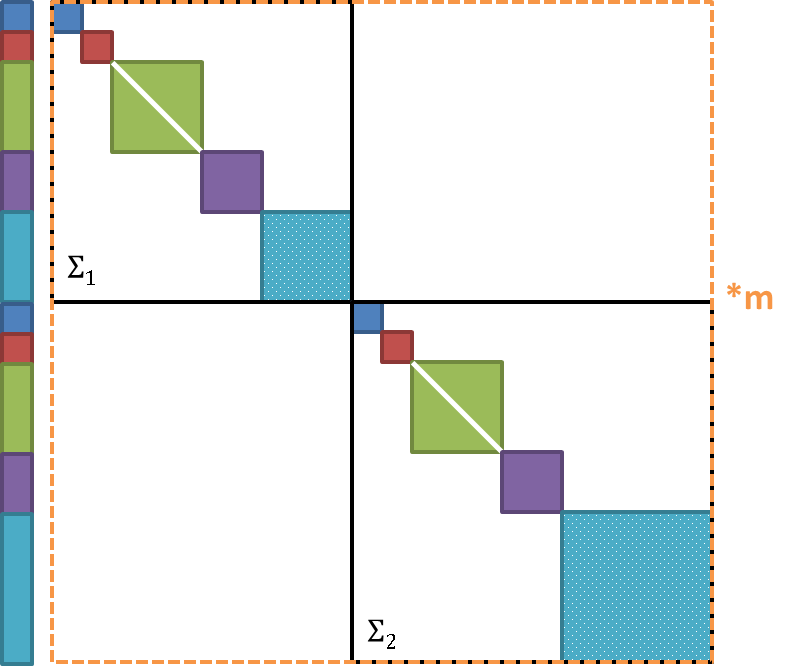
\includegraphics[scale=0.5]{images/CalibrateOne}}
    \subfigure[]{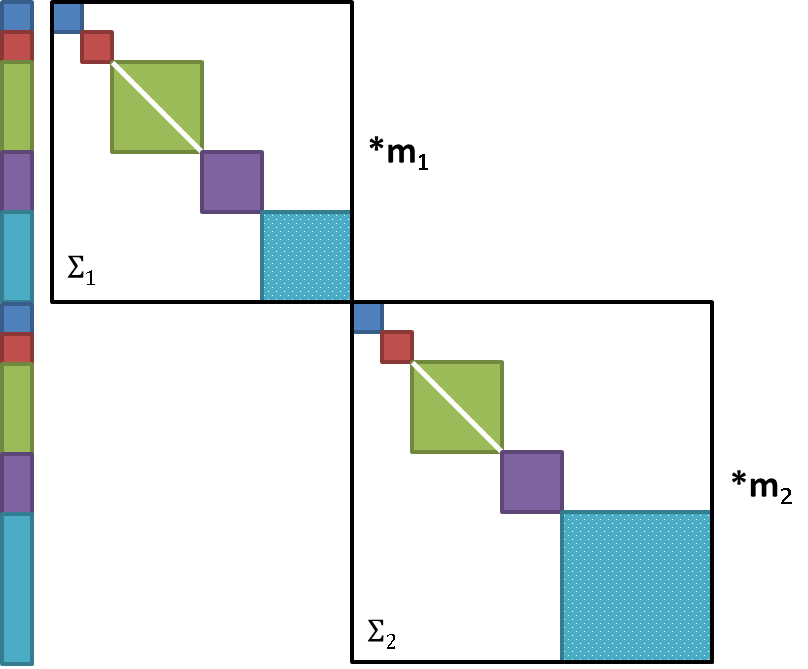
\includegraphics[scale=0.5]{images/CalibratePerExperiment}}
    \subfigure[]{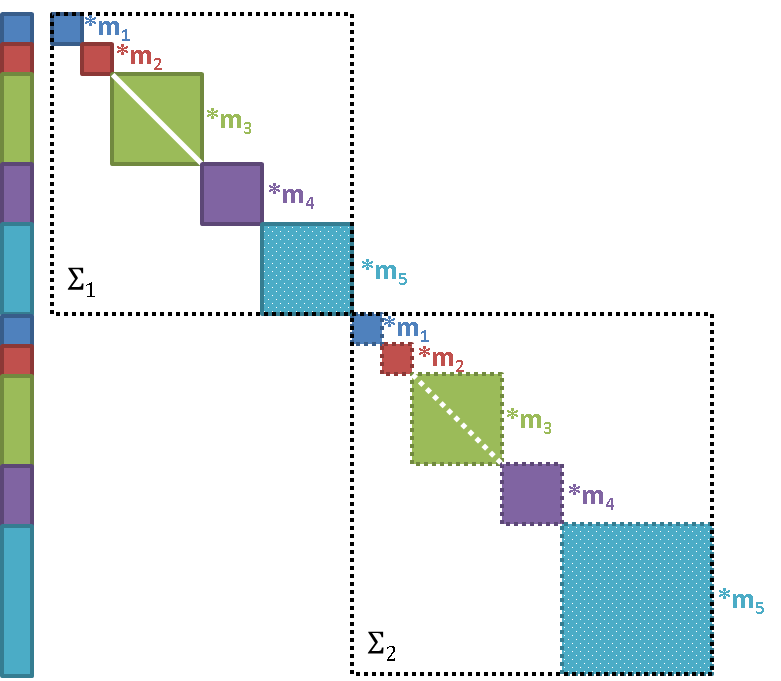
\includegraphics[scale=0.5]{images/CalibratePerResponse}}
    \subfigure[]{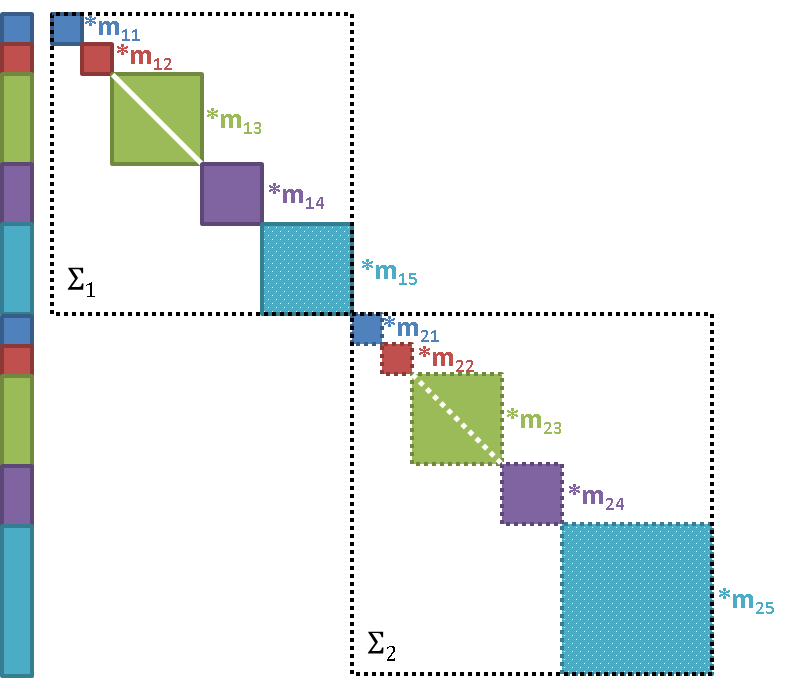
\includegraphics[scale=0.5]{images/CalibrateBoth}}
  \end{subfigmatrix}
  \caption{Calibrating observational error covariance multipliers: (a)
    one multiplier on whole user-provided covariance structure, (b)
    multiplier per-experiment, (c) multiplier per-response, and (d)
    both..}
  \label{fig:uq:obs_err_mult}
\end{figure}

\subsection{Scaling and Weighting of Residuals}

Dakota's scaling options, described in
Section~\ref{opt:additional:scaling}, can be used on Bayesian
calibration problems, using the \dakotakw{calibration_term_scales}
keyword, to scale the residuals between the data points and the model
predictions, if desired. Additionally, Bayesian calibration
residuals-squared can be weighted via the \dakotakw{calibration_terms
weights} specification. Neither set of weights nor scales are adjusted
during calibration.  When response scaling is active, it is applied
after error variance weighting and before \dakotakw{weights}
application. The \dakotakw{calibration_terms} keyword documentation in
the Dakota Reference Manual~\cite{RefMan} has more detail about
weighting and scaling of the residual terms.

\subsection{Model Evidence} 
In some situations, there are multiple models that may represent a phenomenon 
and the user is left with the task to determine which is most appropriate given 
the available data. In this case, Bayesian model selection may help.  Suppose that 
the user has a set of models, $\mathcal{M}$={$M_1,M_2...M_m$} from which to 
choose.  In the Bayesian setting, the parameters of each of these models may be 
updated according to Bayes' rule: 
\begin{equation}
\pi_{post}(\boldsymbol{\theta_i}|D,M_i)=\pi_{prior}(\boldsymbol{\theta_i}|M_i)\frac{\pi(D|\boldsymbol{\theta_i},M_i)}{\pi(D|M_i)}
\end{equation}
where the dependence on the model has been made explicit.  The denominator is used
as the likelihood of a specific model of interest in a version of Bayes' rule which calculates 
the posterior model plausibility as: 
\begin{equation}
\pi_{post}(M_i|D)=\pi_{prior}(M_i)\frac{\pi(D|M_i)}{\pi(D)}
\label{eq:model_plausibility}
\end{equation}
In this equation, the posterior model probability given the data is 
also referred to as model plausibility.  The prior model plausibility, 
$\pi(M_i)$, is usually taken to be uniform, meaning equally likely for all 
models, but it does not have to be.  $\pi(D)$ is a normalizing factor such 
that the sum of all model plausibilities is 1.  In this context, model selection 
involves choosing the model with the highest posterior model plausibility. 
Model evidence is defined as the likelihood in 
Equation~\ref{eq:model_plausibility}, denoted by $\pi(D|M_i)$.  Model evidence 
is determined by averaging the likelihood of its model parameters over all possible 
values of the model parameters, according to their prior distributions.  It is 
also called the marginal likelihood of the model.  Model evidence 
is defined as: 
\begin{equation}
\pi(D|M_i)=\int \pi(D|\boldsymbol{\theta_i},M_i)\pi_{prior}(\boldsymbol{\theta_i}|M_i)d \boldsymbol{\theta_i}
\label{eq:uq:model_evidence}
\end{equation}

There are many ways to calculate model evidence. There are currently two methods 
implemented in Dakota. The user first specifies \texttt{model\_evidence}, then either 
\texttt{mc\_approx} and/or \texttt{laplace\_approx} depending on the
method(s) used to calculate model evidence.
\begin{enumerate}
\item Monte Carlo approximation.  This involves sampling from the prior 
distribution of the parameters, calculating the corresponding likelihood values 
at those samples, and  estimating the integral given in Eq.~\ref{eq:uq:model_evidence} 
by brute force.  The number of samples used in the sampling of the integral is 
determined by \dakotakw{evidence_samples}. Although this method is easy, 
it is not efficient because each sample of the prior density requires 
an evaluation of the simulation model to compute the corresponding likelihood.  
Additionally, many prior samples will have very low (near zero) likelihood, 
so millions of samples may be required for accurate computation of the integral. 
\item Laplace approximation.  This approach is based on the Laplace approximation, 
as outlined in~\cite{Wasserman}.  It has the assumption that the posterior distribution 
is nearly Gaussian, which is not always a safe assumption. 
Then, with maximum a posteriori (MAP) point $\hat{\boldsymbol{\theta}}$, 
the Laplace approximation of model evidence is: 
  
\begin{equation}
\int \pi(D|\boldsymbol{\theta_i},M_i)\pi_{prior}(\boldsymbol{\theta_i}|M_i)d \boldsymbol{\theta_i} \approx \pi(D|\hat{\boldsymbol{\theta}},M_i)\pi(\hat{\boldsymbol{\theta}}|M_i)(2\pi)^{N_i/2}{\|\det(H(\hat{\boldsymbol{\theta}}))\|}^{-1/2}
\end{equation}
where $N_i$ is the number of unknown parameters in the i-th model and 
$H$ is the negative Hessian of the log-posterior evaluated at the MAP point 
$\hat{\boldsymbol{\theta}}$. 
Therefore, this implementation only requires the evaluation of the model likelihood 
and the Hessian of the log-posterior density at the MAP point. 

\end{enumerate}

\subsection{Model Discrepancy}
%kam
Whether in a Bayesian setting or otherwise, the goal of model calibration
is to minimize the difference between the observational data $d_i$ and 
the corresponding model response $q_i(\boldsymbol{\theta})$. In the 
presence of scenario or configuration variables $x$, Eq.~\ref{eq:model} can
be modified,
\begin{equation}
d_i(x) = q_i\left(\boldsymbol{\theta}, x\right) + \epsilon_i,
\end{equation} 
with the ensuing equations of the likelihood and Bayes' Theorem updated 
likewise. The configuration variables represent experimental settings, such 
as temperature or pressure, that may vary between experiments. 

However, it is often the case that the agreement between the 
data and the model after calibration is not sufficiently close. This is 
generally attributed to model form or structural error, and can be corrected 
to some extent with the use of model discrepancy. The Kennedy and 
O'Hagan~\cite{Kenn01} formulation takes the form
\begin{equation}
d_i(x) = q_i\left(\boldsymbol{\theta}, x\right) + \delta_i(x) + \epsilon_i,
\end{equation} 
where $\delta_i(x)$ represents the model discrepancy. For scalar responses, the
model discrepancy is \textit{only} a function of the configuration variables.
Furthermore, one discrepancy model is calculated for \textit{each} observable
$d_i$, $i = 1, \ldots, n$, yielding $\delta_1, \ldots, \delta_n$. For field
responses, a single, global $\delta$ is a function of the configuration 
variables as well as the independent field coordinates, which are usually 
points in time or space. The construction of the model discrepancy in cases 
with mixed scalar and field responses has not been tested.

The current implementation of the model discrepancy capability in Dakota 
serves as a post-processing mechanism after the completion of a Bayesian update.
If \texttt{model\_discrepancy} is specified in the input file, Dakota will 
perform the Bayesian update as detailed in the section above, and then begin 
the process of approximating $\delta$. For each scalar observable $d_i$ and for 
each configuration $x_j$,
\begin{equation}
\delta_i \left( x_j \right) = d_i \left( x_j \right) - 
q_i \left(\boldsymbol{\theta}^*, x_j \right),
\end{equation}
where $\boldsymbol{\theta}^*$ is the average of the calibrated posterior 
distribution of the model parameters. The $i^{th}$ discrepancy function
will be built over the computed $\delta_i \left( x_j \right)$, $j = 1, \ldots,
m$. For field observable $d$, the discrepancy is calculated for each
independent field coordinate $t_{i}$ and for each configuration $x_{j}$,
\begin{equation}
  \delta(t_{i}, x_{j}) = d(t_{i}, x_{j}) - q(\boldsymbol{\theta}^{*}, t_{i},
  x_{j}).
\end{equation}
The global discrepancy function is then built over the computed $\delta(t_{i},
x_{j})$, $i = 1, \ldots, n$, $j = 1, \ldots, m$. For simplicity in future
notation, we let $\delta_{i}(x_i) = \delta(t_i, x_i)$.

The field discrepancy function is built using a Gaussian process regression
model with a quadratic trend function. If instead the responses are scalars, 
more options for the regression model are available. Within the Dakota input 
file, the user may specify the \texttt{discrepancy\_type} to be either a 
Gaussian process or polynomial regression model with the 
\texttt{gaussian\_process} or \texttt{polynomial} commands, respectively. 
Additionally, the order of the trend function may be selected using the 
\texttt{correction\_order} command and choosing one of \texttt{constant}, 
\texttt{linear}, or \texttt{quadratic}. Any specifications using these keywords 
will apply to all $\delta_i$. By default, Dakota will build a Gaussian process 
discrepancy model with a quadratic trend function. Information regarding how 
polynomial and Gaussian process models are built can be found in 
Sections~\ref{models:surf:polynomial} and~\ref{models:surf:kriging}, 
respectively. 

The user may specify new ``prediction" configurations at which the 
corrected model should be calculated. For each response and for each new
configuration, $q_i(\boldsymbol{\theta}, x_{k,new}) + \delta_i(x_{k,new})$ 
will be computed. The prediction configurations can be specified in one of
three ways. If \texttt{num\_prediction\_configs} is included, Dakota will 
uniformly distribute the indicated number of prediction configurations 
throughout the domain of the configuration variable that is given in the 
\texttt{variables} block of the input file. Alternatively, the user may 
explicitly list desired prediction configuration locations within the input
file following the \texttt{prediction\_configs} keyword, or in an external
file to be read in with the \texttt{import\_prediction\_configs} option. If 
none of these three options is selected, Dakota will automatically calculate
corrected model predictions at ten configurations in the scalar response case, 
with the predictions spread uniformly in the configuration variable domain. In 
the case of field responses, corrected model predictions are calculated for each
value of the input configuration variable(s).

Calculations corresponding to each prediction configuration and to each
observable will be output to tabular files. The responses from the discrepancy
model itself is output to \path{dakota_discrepancy_tabular.dat}. Those
from the corrected model are output to \path{dakota_corrected_tabular.dat}.
The user may specify the output file names for the discrepancy and corrected
model tabular files using the \texttt{export\_discrepancy\_file} and
\texttt{export\_corrected\_model\_file} keywords, respectively. 

Variance information corresponding to each specified configuration location 
and for each observable is also computed. In a prediction setting for scalar 
responses, the variance calculated from the discrepancy model is additively 
combined with the variance information provided with the experimental data, 
such that
\begin{equation}
\label{eq:discrep_var}
\Sigma_{total,i}(x) = \Sigma_{\delta, i}(x) + \sigma^{2}_{exp,i} I
\end{equation}
for each observable $i$. Further details of how the variance 
$\Sigma_{\delta,i}(x)$ is computed for Gaussian process and polynomial 
regression models can be found in the Dakota Theory Manual~\cite{TheoMan}. The 
experimental variance provided for parameter calibration may vary for the
same observable from experiment to experiment, thus $\sigma^{2}_{exp,i}$ is
taken to be the maximum variance given for each observable. That is,
\begin{equation}
\sigma^2_{exp,i} = \max_{j} \sigma^2_{i}(x_j), 
\end{equation}
where $\sigma^2_{i}(x_j)$ is the variance provided for the $i^{th}$ observable
$d_i$, computed or measured with the configuration variable $x_j$. 

When each corrected model value $q_i(\boldsymbol{\theta}^{*}, x_{k, new}) +
\delta_i(x_{k,new})$ is considered, the variance calculated 
via~\ref{eq:discrep_var} provides a prediction interval, similar to those 
described in Section~\ref{uq:bayesian:queso}. Including $\sigma^{2}_{exp,i}$ 
in the variance calculation accounts for the uncertainty in the model 
predictions that arise due to uncertainties in the calibration data. These
prediction variances are output to the file 
\path{dakota_discrepancy_variance_tabular.dat} by default. The name of
this file can be modified using the \texttt{export\_corrected\_variance\_file} 
keyword in the input script. If the response is a field, the variance 
information written to this file is the variance of the Gaussian process alone.
Future work includes calculation of combined experimental variance and 
discrepancy model variance for field responses.

Additional details and an illustrative example of these calculations are given 
in the Dakota Theory Manual~\cite{TheoMan}.

\subsection{Bayesian Experimental Design}
\label{sec:bayes_expdesign}

The goal of experimental design is to add observational data to the Bayesian
update that informs model parameters and reduces their uncertainties. In 
Bayesian approaches, data from physical experiments is typically used to 
calibrate a model. However, another common practice is to use responses or
output from a high-fidelity model as ``truth data" in place of experimental 
data in a low-fidelity model calibration. This can be done in with a single
Bayesian calibration, or it can be done iteratively with the use of 
experimental design, where an initial set of high-fidelity runs is 
augmented sequentially to find the next ``best" high-fidelity design point at
which to run the high-fidelity model to add to the calibration data. The 
low-fidelity posterior parameter distribution is then updated again using 
Bayesian calibration. The mutual information is used as the selection criterion 
to guide the process of high-fidelity data acquisition.

In Dakota, design conditions, such as temperature or spatial location, can be 
specified using so-called configuration
variables. The design selection algorithm implemented in Dakota uses a 
user-specified high-fidelity code to produce the ``experimental" or 
observational data that is used in the calibration of the desired low-fidelity 
model. The high-fidelity model is dependent only upon the design or 
configuration variables while the low-fidelity model depends on both the 
design variables and uncertain model parameters. 

An example Dakota input file that implements this Bayesian experimental design 
algorithm is shown in 
Figures~\ref{figure:uq_expdesign1}-\ref{figure:uq_expdesign2}. Note that there 
are three \texttt{model} blocks, one describing the model hierarchy and one 
each for the high-fidelity and low-fidelity models. There are two 
\texttt{variables}, \texttt{interface}, and \texttt{responses} blocks such that 
each model has its own specifications. The low-fidelity \texttt{variables} 
block contains information about both the design variables, which are specified 
with \texttt{continuous\_state}, and the parameters to be updated via Bayes' 
Theorem~\ref{eq:BayesThm}, which are specified using one of the aleatory 
uncertain variable types discussed in Section~\ref{variables:uncertain:cauv}. 
In the high-fidelity \texttt{variables} block, only the 
\texttt{continuous\_state} parameters are included. The specifications of the 
design variables should be consistent in both blocks. Each \texttt{interface} 
block should point to the appropriate high- or low-fidelity code, and the 
\texttt{responses} blocks should contain consistent details about the responses 
from each code. For example, both of the models should return the same number 
of \texttt{calibration\_terms}.  

\stepcounter{figure}
\renewcommand{\thelstlisting}{\thechapter.\arabic{figure}}
\lstinputlisting
[
float=htbp,
lastline=53,
caption={Dakota input file for Bayesian Experimental Design.}, 
label={figure:uq_expdesign1},
captionpos=b,
basicstyle=\small,
frame=single
]
{../../../test/examples-users/bayes_experimental_design.in}
\stepcounter{figure}
\lstinputlisting
[
float=htbp,
firstline=54,
caption={Dakota input file for Bayesian Experimental Design.}, 
label={figure:uq_expdesign2},
captionpos=b,
basicstyle=\small,
frame=single
]
{../../../test/examples-users/bayes_experimental_design.in}

The mutual information experimental design algorithm is selected by specifying 
\texttt{bayesian\_calibration}, \texttt{queso}, and 
\texttt{experimental\_design} within the \texttt{method} block of the input 
file, and the first \texttt{model} block should contain the 
\texttt{hierarchical} specification of the \texttt{surrogate} keyword. The 
algorithm starts by performing a Bayesian calibration using a number of data
points, specified in Dakota by \texttt{initial\_samples}. These initial data
points can be pulled from external data using the 
\texttt{calibration\_data\_file} keyword in the high-fidelity \texttt{response}
block. In this case, \texttt{num\_config\_variables} should be specified and 
set to the number of configuration variables captured in the \texttt{variables} 
blocks. Furthermore, for use in Bayesian experimental design, 
\texttt{calibration\_data\_file} should contain the configuration variables 
and the corresponding high-fidelity model responses. Scalar variance 
information may be included for the calibration data through the use of the 
\texttt{experimental\_variance\_type} or \texttt{simulation\_variance} command 
within the high-fidelity \texttt{responses} block. The former is applied to any 
user-provided data, such as through the \texttt{calibration\_data\_file} 
keyword, while the latter applies only to those high-fidelity model responses 
produced by the high-fidelity code run by Dakota. Further information can be 
found in the Dakota Reference Manual~\cite{RefMan}. If the number of points 
taken from this file is less than \texttt{initial\_samples}, or if no such 
file is provided, Latin Hypercube Sampling is used to draw samples of the 
design space, and the high-fidelity model is run at these points to supplement
the user-specified data. After this initial calibration, a set of design 
conditions (i.e.\ configuration variables) of size \texttt{num\_candidates} is 
proposed. Users may specify these candidate points through the 
\texttt{import\_candidate\_points\_file} command. Again, if the number of 
points in this file is less than \texttt{num\_candidates}, or if no such file 
is provided, Latin Hypercube Sampling is used to draw samples of the design 
space.  

From these candidate designs, that which maximizes the mutual information with
respect to the low-fidelity model parameters is deemed ``optimal." The mutual
information is approximated using the low-fidelity model and a $k$-nearest
neighbor algorithm, as detailed in~\cite{Lew16}. This optimal design is used in 
the high-fidelity model to create a new observation, which is appended to the 
initial data. This updated data is used to recalculate the Bayesian posterior,
and the process repeats until one of three stopping criteria are met.
Multiple optimal designs may be selected concurrently by specifying 
\texttt{batch\_size} in the input script. These designs are selected using
the greedy algorithm described in detail in~\cite{TheoMan}. In this case, the
high-fidelity model is run at all batch-selected optimal designs before the
Bayesian posterior is recalculated with the updated data for an ensuing 
iteration of the experimental design algorithm. 

There are two algorithms that may be used to calculate the mutual information,
both of which are derived in~\cite{Kra04}. The first algorithm discussed 
therein is used as the default algorithm within Dakota; the second may be 
selected by including the keyword \texttt{ksg2} in the Dakota input script. 
Furthermore, the user may choose to include, during the computation of the 
mutual information, a stochastic error term on the low-fidelity model 
responses. This is done by specifying \texttt{simulation\_variance} in the 
\texttt{responses} block corresponding to the low-fidelity model. See the 
Dakota Theory Manual~\cite{TheoMan} for more information regarding the 
implementation of the mutual information calculations.

There are three criteria by which this algorithm is considered complete. 
The user may specify \dakotakw{max_hifi_evaluations}, which limits the number 
of high-fidelity model simulations Dakota will run. Note that this does not 
include any simulations needed to perform the initial Bayesian calibration of 
the low-fidelity model parameters. Alternatively, if the change in the mutual 
information from one iteration to the next is sufficiently small or if all 
candidate points have been exhausted, the algorithm will terminate. 

Progress of the algorithm will be reported to the screen with the rest of the
Dakota output. Furthermore, a summary of the algorithm's results, including, 
for each iteration, the optimal design, the mutual information, and the 
corresponding high-fidelity model response, can be found in the file 
\path{experimental_design_output.txt}.

\subsubsection{One-at-a-time Implementation}

There may be some applications for which the high-fidelity model must be run
independently of Dakota. This algorithm may still be implemented in this case,
however, it requires some extra work by the user to ensure that the 
high-fidelity model information is properly communicated to Dakota, as a 
"dummy" high-fidelity model code must be supplied to Dakota. The data to be 
used in the initial Bayesian calibration should be gathered from the 
high-fidelity model or physical experiment and imported via the 
\texttt{calibration\_data\_file} in the high-fidelity \texttt{responses} block, 
and extra care should be taken to ensure that \texttt{initial\_samples} matches 
the number of experiments in this file. It is also best, for this use-case, to 
use \texttt{import\_candidate\_points\_file}, with \texttt{num\_candidates} 
exactly matching the number of candidate points in the file.

By setting \texttt{max\_hifi\_evaluations} to zero, Dakota will run the initial
calibration of the low-fidelity model, select the optimal design (or multiple
optimal designs when \texttt{batch\_size} is greater than 1) from 
those provided in \texttt{import\_candidate\_points\_file}, and exit 
\textit{without} running the ``dummy" high-fidelity model code. The selected
design(s) will be output to the screen, as well as to 
\path{experimental_design_output.txt}, as detailed above. The high-fidelity
model may then be run offline with the newly selected design point(s).

The user must update \texttt{calibration\_data\_file} with the new 
high-fidelity data when it becomes available, as well as remove the previously
selected design point(s) from \texttt{import\_candidate\_points\_file}. Within 
the Dakota input file, \texttt{initial\_samples}, \texttt{num\_experiments}, 
and \texttt{num\_candidates} should be correspondingly updated. Dakota may then
be run again to yield the next optimal experimental design(s). It should be 
noted that the stopping criteria will not be automatically evaluated by Dakota 
when one-at-a-time implementation is used. The user must determine when the 
algorithm should be terminated.

\section{Uncertainty Quantification Usage Guidelines} \label{usage:uq}

The choice of uncertainty quantification method depends on how the
input uncertainty is characterized, the computational budget, and the
desired output accuracy.  The recommendations for UQ methods are
summarized in Table~\ref{usage:guideuq} and are discussed in the
remainder of the section.

\begin{table}[hbp]
\centering
\caption{Guidelines for UQ method selection.} \label{usage:guideuq}\vspace{2mm}
\begin{tabular}{|c|c|c|}
\hline
\textbf{Method} & \textbf{Desired Problem} & \textbf{Applicable Methods} \\
\textbf{Classification} & \textbf{Characteristics} & \\
\hline
Sampling & nonsmooth, multimodal response functions;       & sampling 
(Monte Carlo or LHS) \\
         & response evaluations are relatively inexpensive & \\
\hline
Local       & smooth, unimodal response functions; & local\_reliability
(MV, AMV/AMV$^2$,\\
reliability & larger sets of random variables;     & AMV+/AMV$^2$+, TANA, 
FORM/SORM) \\
            & estimation of tail probabilities     & \\
\hline
Global      & smooth or limited nonsmooth response; & global\_reliability \\
reliability & multimodal response; low dimensional; & \\
            & estimation of tail probabilities      & \\
\hline
Adaptive    & smooth or limited nonsmooth response; & importance\_sampling, \\
Sampling    & multimodal response; low dimensional; & gpais, adaptive\_sampling, \\
            & estimation of tail probabilities      & pof\_darts \\
\hline
Stochastic & smooth or limited nonsmooth response; & polynomial\_chaos, \\
expansions & multimodal response; low dimensional; & stoch\_collocation\\
           & estimation of moments or moment-based metrics & \\
\hline
Epistemic & uncertainties are poorly characterized &
interval: local\_interval\_est, \\
 & & global\_interval\_est, sampling; \\
 & & BPA: local\_evidence, global\_evidence \\
\hline
Mixed UQ  & some uncertainties are poorly characterized &
nested UQ (IVP, SOP, DSTE) with epistemic \\
 & & outer loop and aleatory inner loop, sampling \\
\hline
\end{tabular}
\end{table}


{\bf Sampling Methods} \\
Sampling-based methods are the most robust uncertainty techniques
available, are applicable to almost all simulations, and possess
rigorous error bounds; consequently, they should be used whenever the
function is relatively inexpensive to compute and adequate sampling
can be performed. In the case of terascale computational simulations,
however, the number of function evaluations required by traditional
techniques such as Monte Carlo and Latin hypercube sampling (LHS)
quickly becomes prohibitive, especially if tail statistics are
needed. %Additional sampling options include quasi-Monte Carlo (QMC)
%sampling and importance sampling (IS),
%or Markov Chain Monte Carlo (MCMC) sampling
%and incremental sampling may also be used to incrementally add samples 
%to an existing sample set.

Alternatively, one can apply the traditional sampling techniques to a
surrogate function approximating the expensive computational
simulation (see Section~\ref{adv_models:sbuq}). However, if this
approach is selected, the user should be aware that it is very
difficult to assess the accuracy of the results obtained. Unlike
the case of surrogate-based local minimization (see
Section~\ref{adv_meth:sbm:sblm}), there is no simple pointwise calculation to
verify the accuracy of the approximate results. This is due to the
functional nature of uncertainty quantification, i.e. the accuracy of
the surrogate over the entire parameter space needs to be considered,
not just around a candidate optimum as in the case of surrogate-based
local. This issue especially manifests itself when trying to estimate
low probability events such as the catastrophic failure of a system.

{\bf Reliability Methods} \\
Local reliability methods (e.g., MV, AMV/AMV$^2$, AMV+/AMV$^2$+, TANA,
and FORM/SORM) are more computationally efficient in general than the
sampling methods and are effective when applied to reasonably
well-behaved response functions; i.e., functions that are smooth,
unimodal, and only mildly nonlinear. They can be used to provide
qualitative sensitivity information concerning which uncertain
variables are important (with relatively few function evaluations), or
compute full cumulative or complementary cumulative response functions
(with additional computational effort). Since they rely on gradient
calculations to compute local optima (most probable points of
failure), they scale well for increasing numbers of random variables,
but issues with nonsmooth, discontinuous, and multimodal response
functions are relevant concerns. In addition, even if there is a
single MPP and it is calculated accurately, first-order and
second-order integrations may fail to accurately capture the shape of
the failure domain. In these cases, adaptive importance sampling
around the MPP can be helpful. Overall, local reliability methods
should be used with some care and their accuracy should be verified
whenever possible.

An effective alternative to local reliability analysis when confronted
with nonsmooth, multimodal, and/or highly nonlinear response functions
is efficient global reliability analysis (EGRA). This technique
employs Gaussian process global surrogate models to accurately resolve
the failure domain and then employs multimodal adaptive importance
sampling to resolve the probabilities. For relatively low dimensional
problems (i.e, on the order of 10 variables), this method displays the
efficiency of local reliability analysis with the accuracy of
exhaustive sampling. While extremely promising, this method is still
relatively new and is the subject of ongoing refinements as we deploy
it to additional applications.

{\bf Adaptive Sampling Methods} \\
There are now a number of methods in Dakota which are tailored to 
estimating tail probabilities.
These methods include both standard importance sampling and 
Gaussian Process Adaptive Importance Sampling, as well as 
adaptive sampling and the POF-darts method. These methods 
are suitable for smooth or limited non-smooth responses, 
and work well in low dimensions. GPAIS and POF-darts utilize 
a Gaussian process surrogate model.  
 
{\bf Stochastic Expansions Methods} \\
The next class of UQ methods available in Dakota is comprised of
stochastic expansion methods (polynomial chaos and stochastic
collocation), which are general purpose techniques provided that the
response functions possess finite second order moments. Further, these
methods capture the underlying functional relationship between a key
response metric and its random variables, rather than just
approximating statistics such as mean and standard deviation. This
class of methods parallels traditional variational methods in
mechanics; in that vein, efforts are underway to compute rigorous
error bounds of the approximations produced by the methods. Another
strength of these methods is their potential use in a multiphysics
environment as a means to propagate the uncertainty through a series
of simulations while retaining as much information as possible at each
stage of the analysis. The current challenge in the development of
these methods, as for other global surrogate-based methods, is
effective scaling for large numbers of random variables. Recent
advances in adaptive collocation and sparsity detection methods
address some of the scaling issues for stochastic expansions.

{\bf Epistemic Uncertainty Quantification Methods} \\
The final class of UQ methods available in Dakota are focused on
epistemic uncertainties, or uncertainties resulting from a lack of
knowledge. In these problems, the assignment of input probability
distributions when data is sparse can be somewhat suspect. One
approach to handling epistemic uncertainties is interval analysis
(\texttt{local\_interval\_est} and \texttt{global\_interval\_est}),
where a set of intervals on inputs, one interval for each input
variable, is mapped to a set of intervals on outputs.  To perform this
process efficiently, optimization methods can be used.  Another
related technique is Dempster-Shafer theory of evidence (Dakota
methods \texttt{local\_evidence} and \texttt{global\_evidence}), where
multiple intervals per input variable (which can be overlapping,
contiguous, or disjoint) are propagated, again potentially using
optimization methods.  The choice between local or global optimization
methods for interval computation is governed by the same issues
described in Section~\ref{opt:usage}.

{\bf Mixed Aleatoric and Epistemic Methods} \\
For problems with a mixture of epistemic and aleatoric uncertainties,
it is desirable to segregate the two uncertainty types within a nested
analysis, allowing stronger probabilistic inferences for the portion
of the problem where they are appropriate. In this nested approach, an
outer epistemic level selects realizations of epistemic parameters
(augmented variables) and/or realizations of random variable
distribution parameters (inserted variables). These realizations
define the objective probabilistic analysis to be performed on the
inner aleatoric level. In the case where the outer loop involves
propagation of subjective probability, the nested approach is known as
second-order probability and the study generates a family of CDF/CCDF
respresentations known as a ``horse tail'' plot.  In the case where
the outer loop is an interval propagation approach
(\texttt{local\_interval\_est} or \texttt{global\_interval\_est}), the
nested approach is known as interval-valued probability (see also
Section~\ref{models:nested}) . In the case where the outer loop is an
evidence-based approach (\texttt{local\_evidence} or
\texttt{global\_evidence}), the approach generates epistemic belief
and plausibility bounds on aleatory statistics.


\begin{comment}
\section{Future Nondeterministic Methods}\label{uq:future}

Uncertainty analysis methods under investigation for future inclusion
into the Dakota framework include extensions to the stochastic
expansion methods and sampling capabilities currently supported.
In particular, smart adaptive methods that can mitigate the curse
of dimensionality are a research emphasis.
%
%Advanced ``smart sampling'' techniques such as bootstrap sampling (BS)
%and Markov chain Monte Carlo simulation (McMC) are being considered.
%We also have an active research focus on adaptive sparse grid methods,
%to more efficiently construct stochastic expansions. 
%
%Efforts have been initiated to allow for non-traditional
%representations of uncertainty. We have implemented Dempster-Shafer
%theory of evidence, and other non-traditional approaches may follow. 
%
We are also currently emphasizing the development of Bayesian methods,
specifically focusing on surrogate-modeling, discrepancy, 
post-processing, and multi-model extensions to the Bayesian
calibration capabilities.
%
%, where a ``prior
%distribution'' on a parameter is updated through a Bayesian framework
%involving experimental data and a likelihood function.
%
%Finally, the tractability and efficacy of the more intrusive
%variant of stochastic finite element/polynomial chaos expansion
%methods, previously mentioned, is being assessed for possible
%implementation in Dakota.
\end{comment}

%%  LocalWords:  MUQ MCMC Langevin
